\chapter{Performance Modeling and Analysis}
\label{ch:perfmodel}
\index{PerfModel!Performance Modeling}
\chaptertoc
\noindent

Generally, work-stealing or reactive load balancing make decisions based on the current execution status at runtime. Their decisions take balancing operation and task migration into account. Balancing operations denote checking imbalance status and exchanging information, while task migration denotes moving tasks from one process to another. These can affect the overall performance. Therefore, it is difficult to determine efficiency as well as performance of balancing decisions before running applications. We address this with a performance model.\\

Regarding the previous works, several performance models for work stealing have been proposed, such as \cite{gast2021analysis}, \cite{tchiboukdjian2010tighter}, \cite{hayat2004dyntimemodelws}. The authors use discrete-time models to address the behavior of work stealing, mainly focusing on the constraints of communication latency when tasks are migrated. In their work, the latency is considered a constant, and all tasks have the same overhead in migration. However, we show that tasks can be different in type and data size in terms of HPC as well as task-based parallel applications. Therefore, communication latency alone cannot model balancing behavior very well in practice, and these models are not suitable in our context. To analyze how the previous models are built, we do not go into detail in this chapter because work stealing has passive behavior from the view of load balancing operations, and it is also extensively analyzed with the existing models mentioned above. Therefore, we summarize one of the most related models in Appendix \ref{App_A:Perf_Model}.\\

In constrast, we introduce a new performance model, mainly focusing on the behaviors of reactive load balancing. We assume a given imbalance context along with the overhead of balancing operations and task migration, where the given imbalance context is already mentioned in Subsection \ref{subsec:dlb}. The overhead is bounded by two metrics, latency ($\lambda$) and delay time ($d$). In detail, the input and output of our model can be simplified as follows.
\begin{itemize}
	\item The main influence inputs include the number of involved processes, number of tasks in total, number of slowdown processes, slowdown factors of corresponding processes, and the overhead for balancing operations as well as task migration (delay time).
	\item The output indicates the performance of modeled and simulated cases in execution time, number of local and migrated (offloaded) tasks on each process.
\end{itemize}

The model is leveraged to design a simulator, where its output can be used to analyze the bound of dynamic load balancing approaches among different scenarios.\\

An overview of this chapter is as follows: Section \ref{sec:NewModel-ReactLB} presents the performance model concerning reactive load balancing, followed by an introduction to the associated simulator and model evaluation in Section \ref{sec:Model-Simulation-Evaluation}. Additionally, Section \ref{sec:Idea-Proactive-LB} highlights the idea of proactive load balancing, which is grounded in our performance model.

\section{A Proposed Model for Reactive Load Balancing in HPC}
\label{sec:NewModel-ReactLB}
\index{PerfModel!A New Performance Model in HPC}

For modeling the performance of dynamic load balancing, we need to understand the behavior associated with balancing operations. For this, we rely on experiments and profiling information to build the model. To stay consistent with the example in Figure \ref{fig:preli_reactlb_operations} on Page \pageref{fig:preli_reactlb_operations}, we highlight the same illustration for reactive balancing behavior in Figure \ref{fig:perfmodel_reactlb_deterministic_estimation}, but we emphasize in detail the steps when task offloading is performed.\\

Figure \ref{fig:perfmodel_reactlb_deterministic_estimation} can be considered as a profiled information of $8$ processes. The y-axis shows $8$ involved processes ($P = 8$), while the x-axis shows execution progress over time steps (time units) from $0$ until termination. In Figure \ref{fig:perfmodel_reactlb_deterministic_estimation}, before tasks are executed, we assume there is a given distribution of $5$ tasks on each process (formulated by $T_{i} = 5$). The performance of each process is expected to be stable, and total load value is balanced. However, the execution speed of processes $P_{4}$, $P_{5}$, $P_{6}$, $P_{7}$ is slowed down, leading to an imbalance at runtime as Figure \ref{fig:perfmodel_reactlb_deterministic_estimation} reveals. With reactive load balancing, each process is deploying a dedicated thread, \texttt{Tcomm}, which is denoted by the dashed line, and the small triangles on each line illustrate reactive operations. For example, at time $t_{6}$ and time $t_{8}$, tasks from the slower processes are offloaded to the faster processes. In terms of two objective factors affecting the decisions of task offloading, we have:
\begin{itemize}
	\item Imbalance level: points to the effect of slowdown on the imbalance ratio.
	\item Reasonable task migration: points to the effect of balancing approach and overhead in balancing operations \& task migration on the offloading decision.
\end{itemize}

\begin{figure}[t]
  \centering
  \includegraphics[scale=0.65]{./pictures/perf_analysis_model/perf_illustration_reactlb_behavior_for_perf_model.pdf}
	\caption{An illustration about the analysis of reactive load balancing based on deterministic estimation.}
	\label{fig:perfmodel_reactlb_deterministic_estimation}
\end{figure}

Following the slowdown affecting execution speed, we formulate the speed of corresponding processes such as speed $S_{P_{0}}$, $S_{P_{1}}$, $S_{P_{2}}$, ..., $S_{P_{7}}$. The total load value of each processes is formulated by load $L_{0}$, $L_{1}$, $L_{2}$, ..., $L_{7}$. In the case of balance, all speed values and their total load values are approximately similar. In the case of imbalance, some speed values are affected by a slowdown factor which we denote by $Slow_{i}$. If $Slow_{i} < 1.0$, it can make the execution speed of process $P_{i}$ slower. For example, the expected speed of process $P_{i}$ is $S_{P_{i}} = 1.0$ (can be simplified as $1$ task/time unit). When it is slowed down by $50\%$ ($\times 0.5$), the execution speed would be $0.5$ task/time unit. Otherwise, if $Slow = 1.0$, the execution speed is not changed. For mapping slowdown to the execution time of a task, assuming a time unit is in seconds, then the execution of a task takes one second ($1s$) if the speed $S_{P_{i}}$ is $1.0$ task/second. If $Slow_{i} = 0.5$ affects the speed $S_{P_{i}}$, that task needs $2s$ to be finished.\\

In a specific context, when we can analyze the impact of slowdown factor on imbalance levels by keeping a given distribution of tasks and a number of involved processes, then varying slowdown factor as well as the number of slowdown processes. For changing the $Slow_{i}$ values, we can formulate its impact on speed $S_{P_{i}}$ and load $L_{i}$ by Equation \ref{eq:slowdown_impact_speed_and_L}.

\begin{equation} \label{eq:slowdown_impact_speed_and_L}
\begin{split}
	Slow_{i} & \overset{impact}{\rightarrow} S_{P_{i}}: S_{P_{i}} \times Slow_{i} \\
	Slow_{i}' = \frac{1}{Slow_{i}} & \overset{impact}{\rightarrow} L_{i}: L_{i} \times Slow_{i}'
\end{split}
\end{equation}

In Equation \ref{eq:slowdown_impact_speed_and_L}, $Slow_{i}$ affects directly execution speed, and the value of $S_{P_{i}}$ can be decreased. $Slow_{i}'$ affects directly the total load value at the end; therefore, the value of $L_{i}$ can be increased. Taking the case in Figure \ref{fig:perfmodel_reactlb_deterministic_estimation} for instance, we assume the total load values of all processes are multiplied with an array of $Slow_{i}'$ values. Then, the slowdown at runtime makes them unbalanced and $R_{imb}$ is calculated along with $Slow_{i}'$. Note that load $L_{i}$ without performance slowdown are expected equally; therefore, we can assume that load $L_{0}$ $\approx$ $L_{1}$ $\approx ... $ $L_{7}$ and $\approx$ $L$. In average, the total load values and imbalance ratio can be calculated by Equation \ref{eq:unexpected_imb_8_ranks}.

\begin{equation} \label{eq:unexpected_imb_8_ranks}
\begin{split}
	L_{max} &= \text{max}(L_{0} \times Slow_{0}', ..., L_{7} \times Slow_{7}') \\
	L_{avg} &= L \times \frac{Slow_{0}' + ... + Slow_{7}'}{P}, \text{where } L \approx L_{0} \approx ... \approx L_{7}) \\
	R_{imb} &= \frac{L \times Slow_{max}'}{L \times \frac{Slow_{0}' + ... + Slow_{7}'}{P}} - 1\\
	        &= \frac{P \times Slow_{max}'}{\sum_{i=0}^{P-1} Slow_{i}'} - 1
\end{split}
\end{equation}

The following estimation analyzes two common cases of slowdown effects.\\

\begin{figure}[t]
  \centering
  \includegraphics[scale=0.625]{./pictures/perf_analysis_model/perf_heatmap_slowdown_impact.pdf}
	\caption{The impact of slowdown values on load imbalance ratios.}
	\label{fig:heatmap_slowdown_impact}
\end{figure}

\noindent \textbf{Case 1:} Slowdown remains constant during execution, and this happens on some processes, which are called slowdown processes. The slowdown values among processes can be different. However, to easily show the slowdown effect changing over its values and over the number of involved processes, Figure \ref{fig:heatmap_slowdown_impact} highlights an estimation by two heatmaps, where one on the left shows the heatmap color of imbalance ratio ($R_{imb}$) and one on the right shows the color of standard deviation ($std$). Each figure is labeled on the horizontal axis with the number of slowdown processes (such as $num.p.1$, $num.p.2$, ..., $num.p.8$), and on the vertical axis with the factor of slowdown (such as $2\times$, $3\times$, ..., $9\times$). The experiments in Figure \ref{fig:heatmap_slowdown_impact} are stayed with $8$ processes. As an example, $num.p.1$ indicates that one of $8$ processes is slowed down, while $2\times$ indicates the slowdown factor in that process is $2$ times compared to the stable processes. Depending on the color of the heatmap, we determine an imbalance ratio corresponding to a standard deviation. For example, in the case of $num.p.1$ and $2\times$, the imbalance ratio is $0.8$, corresponding to a standard deviation of $8.3$. The value of standard deviation indicates load dispersion between different processes.\\

\begin{figure}[t]
  \centering
  \includegraphics[scale=0.45]{./pictures/perf_analysis_model/perf_analysis_deterministic_model_imb_cases.pdf}
	\caption{Three imbalance scenarios when only one process is slowed down.}
	\label{fig:three_imb_situations_with_one_slow}
\end{figure}

As can be seen, bad situations occur when slowdown cases happen only in a few processors/cores corresponding to the mapped processes or threads. The worst in this example is when one process is significantly slowed down. Figure \ref{fig:three_imb_situations_with_one_slow} highlights three imbalance scenarios with $R_{imb}$ $=$ $2.0$, $3.0$, $4.0$ (named accordingly Scenario 2.0, Scenario 3.0, Scenario 4.0), where only process $P_{7}$ is slowed down. If tasks are migrated to balance the load, only process $P_{7}$ should offload tasks to others.\\

\noindent \textbf{Case 2:} Slowdown is unpredictable, where $Slow_{i}$ is varied during execution. Assume that the execution example is still stayed with $8$ processes as in Figure \ref{fig:perfmodel_reactlb_deterministic_estimation}, we perform the execution running over $100$ iterations, where the slowdown values are randomized over each iteration. Figure \ref{fig:randomized_slowdown} shows an estimation of Case 2 with both lines: imbalance ratio ($R_{imb}$) and standard deviation ($std$). The x-coordinate denotes the indices of iterations; the left and right y-coordinates denote imbalance ratio and standard deviation respectively. If the uncertainty of slowdown is high, this leads to a challenge in load prediction and dynamic load balancing. Particularly, it is difficult to propose a good strategy for migrating tasks.\\

\begin{figure}[t]
  \centering
  \includegraphics[scale=0.45]{./pictures/perf_analysis_model/perf_double_line_random_slowdown.pdf}
	\caption{Randomized slowdown and unpredictable imbalance ratios over 100-iterations execution.}
	\label{fig:randomized_slowdown}
\end{figure}

In practice, Case 1 and Case 2 might be overlapped except when the fluctuation level of Case 2 is too high. Case 2 usually happens when our computing resources are over-subscribed by sharing between different programs simultaneously. Otherwise, Case 1 occurs more often in parallel compute clusters because of the inherent variation of chip design today, such as variation in power and temperature of the chips. Acun et al. \cite{acun2016variturboboost} have shown similar experiments like Case 1 caused by the variation among processors on the Turbo Boost-enabled supercomputers (an execution time difference of up to $16\%$). The other works from \cite{weisbach2018hwvariation} \cite{tuncer2019onlinediagvar} have introduced the methods and tools to characterize hardware performance variation, even reproduce performance variations for research purposes \cite{ates2019hpas}. In addition, not only CPUs, similar analyzes are also performed on current GPU architectures \cite{yoshida2022perfvargpu}.\\

%The estimation of these two cases shows how much slowdown can impact the level of load imbalance.\\ 

Following a given imbalance level, the next subsection introduces how the overhead in balancing operation and task migration can affect the decision of task offloading. Typically, we show an estimation of the maximum number of tasks that need to be exchanged to balance the load in a specific situation.

% ----------------------------------------------------
% Deterministic Estimation in average
% ----------------------------------------------------
\subsection{Deterministic Estimation} \label{subsec:deterministic_estimation}

Deterministic estimation aims at calculating on average for how many tasks can be offloaded. For example, we have a given imbalance ratio, a number of involved processes which we know overloaded and underloaded processes. Then, according to the overhead of task migration, we can estimate how many tasks should be migrated. The model for deterministic estimation provides an overview in advance about how task migration is limited in a specific case and in a specific system.\\

% ---------------------------------
% insert an inline figure here
% ---------------------------------
\begin{figure}[t]
  \centering
	\includegraphics[scale=0.8]{./pictures/perf_analysis_model/perf_inline_fig_Li_and_Tcomm.pdf}
	\caption{Three main operations driven by reactive load balancing and total load value afterward.}
	\label{fig:detailed_Tcomm_operations_and_L}
\end{figure}

Before a task is migrated, there are three main operations driven by the reactive load balancing approach, including monitoring execution status, exchanging status, and offloading tasks. These operations are performed by $Tcomm$ at runtime and shown as $T_{\text{monitor}}$, $T_{\text{info\_exchange}}$, and $T_{\text{offload}}$ in Figure \ref{fig:detailed_Tcomm_operations_and_L}. The line of $Tcomm_{i}$ illustrates balancing operations according to process $P_{i}$. Because these three operations cause the most overhead that we count for an impact on reactive load balancing; therefore, we name $T_{\text{monitor}}$ to indicate the time of monitoring operation, $T_{\text{info\_exchange}}$ for the time of current execution status (queue status) exchange, and $T_{\text{offload}}$ for the time of task offloading. Following that, tasks might be migrated or not migrated over time progress. We imply that the value of $T_{\text{monitor}}$, $T_{\text{info\_exchange}}$, $T_{\text{offload}}$ might be varied during execution, depending on a given time and data size of migrated tasks.\\

In Figure \ref{fig:detailed_Tcomm_operations_and_L}, we also highlight the line of $L_{i}$ to denote the final load value of the corresponding process $P_{i}$. Load $L_{i}$ is a sum of the wallclock execution time values of tasks, including local and remote tasks. Local tasks (green rectangles) are associated with the load values, while remote tasks (yellow rectangles) are related to the remote load values, where remote tasks indicate the tasks received from the other processes. Overall, the operations and load values shown in Figure \ref{fig:detailed_Tcomm_operations_and_L} are formulated in Equation \ref{eq:form_L_and_Tcomm}.

\begin{equation} \label{eq:form_L_and_Tcomm}
	\begin{cases}
		Tcomm_{i} = T_{\text{monitor}} + T_{\text{info\_exchange}} + T_{\text{offload}} \\
		L_{i} = \sum_{j \in T^{'}_{i}} w_{j}^{\text{local}} \pm \sum_{k=0}^{k_{i}} w_{k}^{\text{remote}}
	\end{cases}
\end{equation}

The number of local tasks of the original process might not be the same as before execution if we perform reactive load balancing. Therefore, in $\sum_{j \in T^{'}_{i}} w_{j}^{\text{local}}$, $T_{i}^{'}$ is the new set of local tasks belonging to process $P_{i}$, value $w$ with ``$\text{local}$'' indicates the wallclock execution time of local tasks. In $\sum_{k=0}^{k_{i}} w_{k}^{\text{remote}}$, ``$\text{remote}$'' indicate remote tasks. The value of $k_{i}$ represents the total number of tasks offloaded to process $P_{i}$. If process $P_{i}$ is the one offloading tasks, the sign will be negative ($-$) for $\sum_{k=0}^{k_{i}} w_{k}^{\text{remote}}$. With all migrated tasks, we use $K$ to denote the total number between all involved processes. For example, with the number of $P$ processes in total, $K$ $=$ $k_{0}$ $+$ $k_{1}$ $+$ $k_{2}$ $+$ $...$ $+$ $k_{P-1}$, where obviously if a process does not receive remote tasks, then the corresponding $k_{i}$ value is zero. The main idea of deterministic estimation is to estimate $K$ in general.\\

There are two bounds estimated, average bound and maximum bound. The average bound relies on the average load of accumulative overloaded and underloaded values, while the maximum bound relies on the maximum and minimum load values of corresponding processes.\\

\noindent \textbf{Average Bound:} revolves around the difference of total load values among processes to calculate overloaded and underloaded values. We assume that the total overloaded value must fill the gap between average and underloaded values.

\begin{itemize}
	\item Theoretically, the ideal balance is average load value ($L_{avg} = \text{average}(L_{i}), \forall i \in P$).
	\item The sum of overloaded values should be equal to the sum of underloaded values, $\sum L_{\text{overloaded}} = \sum L_{\text{underloaded}}$, where
			\begin{equation} \label{eq:L_over_under_load}
				\begin{cases}
					\sum L_{\text{overloaded}}  &= \sum_{i \in P} (L_{i} - L_{avg}) \mid L_{i} > L_{avg} \\
					\sum L_{\text{underloaded}} &= \sum_{i \in P} (L_{avg} - L_{i}) \mid L_{i} < L_{avg}
				\end{cases}
			\end{equation}
	\item To balance the gap between $\sum L_{\text{overloaded}}$ and $\sum L_{\text{underloaded}}$, suppose $K$ tasks are migrated.
\end{itemize}

\noindent $K$ tasks are offloaded to the number of underloaded processes denoted by $M$. Following $M$, the number of overloaded processes is $P-M$. Alternatively, we use $P_{underloaded}$ to indicate the number of underloaded processes and $P_{overloaded}$ for the number of overloaded processes, where $P_{overloaded} = P-M$. If the sum of data size of $K$ tasks is denoted by $S_{\text{transfer}}$ and the sum of delay time values for offloading $K$ tasks is $D$, then we can estimate how much $K$ is bounded. This bound is under the constraints: a given latency ($\lambda$) and an average bandwidth ($\overline{B}$). In detail, $S_{\text{transfer}} = \sum_{i \in K} s_{i}$, and $D = \sum_{i \in K} d_{i}$, where $s_{i}$ is the data size of task $i$ and $d_{i}$ is the delay time calculated by $\lambda + \frac{s_{i}}{B_{i}}$; $B_{i}$ is the bandwidth at the time task $i$ is offloaded.\\
			
Simply put of $\overline{s}$ as the average data size for each task, the total delay time of offloading $K$ tasks should not exceed the ratio between $\sum L_{\text{overloaded}}$ and $M$. This is considered as a gap for filling the underloaded load. Equation \ref{eq:average_bound} shows the bound of $K$ limited by this ratio, implying the total overloaded value sharing across $M$ underloaded processes.

\begin{equation} \label{eq:average_bound}
	\begin{cases}
		K \times (\lambda + \frac{\overline{s}}{\overline{B}}) &\leq \frac{\sum L_{overloaded}}{M} \\
		\Leftrightarrow K   &\leq \frac{\sum L_{overloaded}}{(\lambda + \frac{\overline{s}}{\overline{B}}) \times M} \\
		\Leftrightarrow K   &\leq \frac{\sum L_{overloaded}}{\overline{d} \times M}, \text{where } \overline{d} \text{ is the average delay time per task migration}
	\end{cases}
\end{equation}

\noindent Based on the estimation model in Equation \ref{eq:average_bound}, we show an illustration of how it works with the latency and bandwidth information from real HPC clusters. The example is kept the same with $8$ processes. For a specific imbalance scenario, we assume there are two slowdown processes. The slowdown factor is set $5\times$ slower than normal processes, and $R_{imb}$ is about $1.5$. \\

\begin{figure}[t]
  \centering
  \includegraphics[scale=0.65]{./pictures/perf_analysis_model/perf_analysis_avg_bound_principle_case_1.5_two_sld_procs.pdf}
	\caption{An illustration of deterministic estimation on average.}
	\label{fig:explain_avg_bound_for_situation_1}
\end{figure}

This scenario is illustrated in Figure \ref{fig:explain_avg_bound_for_situation_1}. The chart on the left side shows $8$ processes from $P_{0}$ to $P_{7}$ along with their total load values. The $L_{avg}$ value is determined by the dashed line, \textit{ideal balanced}. The chart on the right side highlights the total overloaded value of process $P_{0}$ and process $P_{1}$, which is fairly shared to $6$ underloaded processes, $M=6$. Hence, we can estimate how much time and how many tasks ($K$) are limited for migration. The scenario here represents the number of overloaded processes smaller than the number of underloaded processes, $P_{\text{overloaded}} < P_{\text{underloaded}}$.\\

% --------------------------------------------------------
\newpage
% --------------------------------------------------------

Expanding this scenario, we emphasize two more scenarios that are summarized as follows.

\begin{itemize}
	\item Scenario 1: is explained above and shown in Figure \ref{fig:explain_avg_bound_for_situation_1}. The slowdown factor is $5\times$, the number of slowed down processes is $2$, and $R_{imb} = 1.5$. This scenario shows the number of overloaded processes smaller than the number of underloaded processes, $P_{\text{overloaded}} < P_{\text{underloaded}}$.
	\item Scenario 2: the slowdown factor is also $5\times$, the number of slowed down processes is $4$, $R_{imb} = 0.7$, and $P_{\text{overloaded}} = P_{\text{underloaded}}$.
	\item Scenario 3: the slowdown factor is set $\approx 8\times$, the number of slowed down processes is $6$, $R_{imb} = 0.3$, and $P_{\text{overloaded}} > P_{\text{underloaded}}$.
\end{itemize}

The corresponding latency and bandwidth information is collected from three different HPC clusters. We use the average $\lambda$ and $\overline{B}$ measured from CoolMUC2\footnote{https://doku.lrz.de/display/PUBLIC/CoolMUC-2 \label{footnote:lrz_coolmuc}}, SuperMUC-NG\footnote{https://doku.lrz.de/display/PUBLIC/SuperMUC-NG \label{footnote:lrz_sng}}, and BEAST\footnote{https://www.lrz.de/presse/ereignisse/2020-11-06\_BEAST/ \label{footnote:lrz_beast}} at Leibniz Supercomputing Centre (LRZ). These systems are also used to perform experiments in the following sections. CoolMUC2 has 28-way Intel Haswell-based nodes and an FDR14 Infiniband interconnect. SuperMUC-NG features Intel Skylake compute nodes with 48 cores per dual-socket, using Intel OmniPath interconnection. In BEAST system, the compute nodes are connected via a higher interconnect bandwidth, HDR 200Gb/s InfiniBand.\\

\begin{figure}[t]
  \centering
  \includegraphics[scale=0.4375]{./pictures/perf_analysis_model/perf_k_offload_tasks_vs_delay_avg_bound.pdf}
	\caption{Estimation of $K$ offloaded tasks on average under the constraints of delay time, imbalance level, task data size, and the number of slowdown processes in task migration.}
	\label{fig:k_estimation_avg_bound}
\end{figure}

The average latency $\lambda$ and bandwidth $\overline{B}$ of CoolMUC2 (\texttt{coolmuc2}), SuperMUC-NG (\texttt{sng}), and BEAST system (\texttt{beast}) are shown in Figure \ref{fig:k_estimation_avg_bound} (A), measured by OSU Benchmark \cite{panda2021mvapich}. The benchmark is run on each cluster with two nodes, and the basic communication interface is MPI point-to-point. The x-axis shows message sizes from 128 bytes to 256 MB that can account for the data size of tasks during migration. The left y-axis shows bandwidth in $MB/s$, while the right y-axis shows latency in $\mu$s. As a result, BEAST has the best communication performance, while CoolMUC2 is the worst due to different interconnection technologies. \\

In Figure \ref{fig:k_estimation_avg_bound} (B), (C), (D), we show the results of $K$ estimation associated with the mentioned scenarios $1$, $2$, $3$. Following the x-axis, we show the task sizes from $400$ KB to $78919$ KB (almost $80$ MB), which are enough to highlight the trend of $K$ estimation and to represent the data sizes of each task in common task-based parallel applications. The y-axis shows the $K$ values, representing the maximum number of tasks that we can offload under the constraints of $\sum L_{\text{overloaded}}$, $\lambda$, and $M$. In Figure \ref{fig:k_estimation_avg_bound} (B), $R_{imb}$ is $1.5$, and two processes are slowed down. The total overloaded value is from process $P_{0}$ and process $P_{1}$, where we share this amount of load over $6$ victim processes. We highlight that the migration time of tasks should not exceed the shared value shown as the constraint segment over migration time in Figure \ref{fig:explain_avg_bound_for_situation_1}.\\

Similarly, Figure \ref{fig:k_estimation_avg_bound} (C) and (D) show that $K$ is decreased when the data size of tasks increases. The value of $K$ still reaches thousands tasks if we offload the tasks continuously, in particular with the size $\approx$ $80$ MB. This shows that communication overhead for task migration in distributed memory might not be the most influential factor. There might be some impacts from the other factors in balancing operations before a task can be migrated. Besides that, $K$ estimated in this bound relies on the average of accumulative overloaded and underloaded values. In the following paragraph, $K$ estimation is conducted in the bound of maximum overloaded and minimum underloaded values, which might stretch the constraint segment of migration time and $K$ may be more than the average bound. \\

\begin{figure}[t]
  \centering
  \includegraphics[scale=0.65]{./pictures/perf_analysis_model/perf_analysis_minmax_bound_principle_case_1.5_two_sld_procs.pdf}
	\caption{An illustration of deterministic estimation on min-max load values.}
	\label{fig:explain_minmax_bound_for_situation_1}
\end{figure}

\noindent \textbf{Min-Max Bound:} simply revolves around the maximum (max) and minimum (min) load values of corresponding processes. Min-max implies the longest way to offload tasks between the most overloaded and the most underloaded processes. Their difference can represent the effect of delay time in task migration.\\

Figure \ref{fig:explain_minmax_bound_for_situation_1} illustrates estimating $K$ based on the most overloaded and underloaded process. The longest way is between process $P_{0}$ and process $P_{7}$, which dominates the most time progress for offloading tasks. Then, we cut a half of the load difference to share each other. The min-max bound of estimating $K$ is summarized as follows.

\begin{itemize}
	\item The difference between the min and max load values is denoted by $\Delta_{max-min} = L_{max} - L_{min}$.
	\item Based on $\Delta_{max-min}$, we estimate $K$ as the number of offloaded tasks. Similarly, the assumption about data size in migrating tasks is kept the same as average bound.
	\item  The bound of $K$ is calculated by
\end{itemize}

\begin{equation} \label{eq:minmax_bound}
	\begin{cases}
		K \times (\lambda + \frac{\overline{s}}{\overline{B}}) &\leq \frac{\Delta_{max-min}}{2} \\
		\Leftrightarrow K  &\leq \frac{\Delta_{max-min}}{2 \times (\lambda + \frac{\overline{s}}{\overline{B}})} \\
		\Leftrightarrow K  &\leq \frac{\Delta_{max-min} \times \overline{B}}{2 \times (\lambda \times \overline{B} + \overline{s})}
	\end{cases}
\end{equation}

\begin{figure}[t]
  \centering
  \includegraphics[scale=0.4375]{./pictures/perf_analysis_model/perf_k_offload_tasks_minmax_bound.pdf}
	\caption{The estimation of $K$ offloaded tasks under the constraints of delay, imbalance level, and task size with the bound of min-max load difference.}
	\label{fig:k_estimation_minmax_bound}
\end{figure}

The results of $K$ estimation are revealed in Figure \ref{fig:k_estimation_minmax_bound}. With the given latency and delay time on three corresponding clusters, the bound of $K$ is higher than the average bound. Likewise, $K$ is still high if we continuously perform offloading tasks during execution.\\

In practice, most analyses and hypotheses suggest that the impact of communication overhead on task migration contributes to slow work stealing as well as reactive load balancing. However, we show that task migration overhead is not only the most influential factor if we perform offloading tasks continuously. These estimations motivate a more in-depth analysis between task migration overhead and balancing operation overhead. The overhead of balancing operations includes the time of monitoring load, exchanging information, and calculating imbalance ratio before we decide to offload a task. The following subsection will show how they impact task offloading decisions.

% On the side of dedicated threads, $Tcomm_{i}$ is bounded by the bottleneck process with the maximum load. With $T_{\text{offload}}$ we can estimate the number of offloaded tasks ($K$) as an upper bound for $\sum_{k=0}^{K} w_{k}^{\text{remote}}$.

% The idea is to see, in general, how many tasks can be offloaded and how much balance we can improve with the given information. Following this, we briefly recall the context in this thesis alongside. The problem gives $T$ tasks in total distributed on $P$ processes. After a distribution, each process is assigned a set of tasks, $T_{i}$ for process $i$. Corresponding to $T_{i}$, the total load of each process is $L_{i}$. To facilitate modeling, we define each task belonging to a set $T_{i}$ with a weight of execution time $w_{j}, \forall j \in T_{i}$. In the case of non-interference during execution, the total load per process is $L_{i} = \sum_{j \in T_{i}} w_{j}$.\\

%As we can see, the context of unexpected imbalance looks simple. However, many factors can make it difficult to work at runtime, e.g., the level of ($R_{imb}$), the number of underloaded or overloaded processes, task data in migration, delay time. Step by step, the deterministic model estimates the performance as follows,
%\begin{enumerate}[label=\arabic*)]
%	\item Given $P$ processes, $T$ tasks in total.
%	\item Following a given distribution, each process holds a set $T_{i}$ tasks corresponding to a total load value $L_{i}$, where $\forall i \in P$.
%	\item For performance slowdown at runtime, $L_{max}$, $L_{min}$, $L_{avg}$ are defined as the maximum, minimum, and average load respectively. The imbalance ratio is calculated by $R_{imb} = \frac{L_{max}}{L_{avg}} - 1$, where $L_{max}$ is considered to define the makespan or completion time.
%	\item Without load balancing, the performance model on each process is $L_{i} = \sum_{j \in T_{i}} w_{j}$. The $L_{i}$ value indicates the load of local tasks belonging to the original process.
%	\item With load balancing, the communication thread ($Tcomm_{i}$) runs along with the other execution threads to monitor load and offload tasks. It partially overlaps communication \& computation. Therefore, we also count it inside the model. The average load value ($L_{avg}$) is concerned as an optimal value of balance. Reactively, tasks from the \textit{overloaded} rank (who has load $> L_{avg}$) are offloaded to the corresponding \textit{underloaded} rank (who has load $< L_{avg}$). Following that, we define the model below.

%			Inside $Tcomm_{i}$, we spend time or so-called overhead for monitoring load/execution speed ($T_{\text{monitor}}$), task offloading ($T_{\text{offload}}$), and monitored information exchange ($T_{\text{info\_exchange}}$). The inline figure shows why we have these terms in the model. The idea comes from the behavior of reactive task offloading or even work stealing. Before a task is migrated, we have to perform several operations, e.g., check the status, share information, and calculate the imbalance condition. They also take time to manage and might lead to late decision-making. Each process has a dedicated $Tcomm_{i}$, which runs along with the main execution. Therefore, $L_{i}$ will be affected when task offloading happens or imbalance conditions meet. Besides, these reactive operations occur repeatedly and dynamically that might show: $T_{\text{monitor}}$, $T_{\text{info\_exchange}}$, $T_{\text{offload}}$ slots are interleaved. The task offloading is unlikely to satisfy the condition to occur continuously.
%\end{enumerate}

%However, the imbalance problem might happen at runtime because of performance slowdown on some processors. For applying reactive load balancing, one dedicated thread per process will run asynchronously with the other execution threads. To model this behavior, we assume discrete execution time regulated by steps such as a time unit.
%
%The communication in HPC systems is challenging to predict how the variability changes. A part of this is due to the physical and virtual distance between nodes in large-scale distributed computing systems. Communication and task transfer activity among them cannot be assumed instantaneous. Thus, the information that a particular node has about other nodes at any time is dated and may not accurately represent the current state of the other nodes.\\
%
%The previous section shows a related performance model for work stealing and latency. The authors highlight how the latency can impact an upper bound of optimizing makespan. Nevertheless, there are still further problems with delay time in practice. Besides, we also need further analysis in modern architectures and new parallel programming paradigms. In detail, we address some opinions to motivate our proposed performance model as follows.
%\begin{itemize}
%	\item The existing models focus on latency which is considered as a constant time between sending and receiving the head of a message. This might imply that the migration time of tasks will be the same, not completely reflected in practice. Because we consider task migration time to be affected by latency, bandwidth, and message size at a time. If there are no conflicts, the transmission time (delay $d$) can be calculated by $d = \lambda + \frac{s}{B}$, where $d$ is delay, $\lambda$ is latency, $s$ and $B$ are message size, network bandwidth.
%	\item In terms of modern architectures and current programming models such as task-based paradigms, a process can have multiple execution threads, and one can be dedicated to communication. This paradigm can overlap communication and computation overhead. The dedicated thread can reduce time delay and perform asynchronously while other threads execute tasks. However, its behavior might be incorrect just due to the time delay in deciding the victim and tasks for offloading.
%\end{itemize}
%
%The above opinions generally motivate us to a performance model for work stealing or reactive load balancing approaches with delay time. ``Reactive'' means that we do not need to wait for the idle processes, and tasks will be considered for migration in advance. Therefore, we call reactively offload tasks from a slow process to a fast one asynchronously if an imbalance condition meets. The reactive idea can work in a distributed memory system. This section will mainly focus on reactive fashion and introduce a new model to analyze it. The model's target is to estimate an upper bound of task offloading under the input constraints of imbalance level, number of task distribution, and delay in task offloading. Figure \ref{fig:perfmodel_reactlb_behavior} shows again the illustration of reactive load balancing with task offloading behaviors.\\
%
%\begin{itemize}
%	\item Each process has a dedicated thread that monitors execution speed and offloads tasks around when the imbalance condition is met.
%	\begin{itemize}
%		\item Execution speed monitoring: this information depends on how we define it. Traditionally, we count the number of remaining tasks per queue to get the status of each process (or so-called MPI rank). The values reflect $T_{i}(t)$ at time $t$.
%		\item Imbalance condition: we can also rely on $T_{i}(t)$ at a time to calculate $R_{imb}$ if there is no prior knowledge about load.
%	\end{itemize}
%	\item Number of offloaded tasks at a time: without prior knowledge, this value can be set based on a specific strategy. For a safe threshold, it should be one task at once. Therefore, $O_{ij}(t) = 1$ indicates that Process $i$ offloads $1$ task to $j$ at time $t$.
%	\item $Tcomm$ should terminate after the bottleneck process (which holds $W_{par}$ or the makespan) finishes.
%\end{itemize}
%
%To ease modeling, we approach two ways of model formulation. One is a deterministic model based on the assumption about the given distribution of tasks over processes without time progress. The other is a discrete-time model, including a decreased function of the queue length over time on each process.

% ----------------------------------------------------------
% Remarked questions or emaphasized hypothesis/opinions
% ----------------------------------------------------------
%\begin{shaded}
%	\noindent How performance slowdown impact imbalance ratio?
%\end{shaded}

% ----------------------------------------------------------
% Remarked questions or emaphasized hypothesis/opinions
% ----------------------------------------------------------
%\begin{shaded}
%	\noindent How does the average bound work with real system information?
%\end{shaded}

% ----------------------------------------------------
% Discrete Time Model in detail
% ----------------------------------------------------
\subsection{Discrete Time Model} \label{subsec:discrete_time_model}

The idea of discrete-time models is to break execution time progress into time steps. In our work, we aim to model the behaviors of reactive load balancing based on queue length over time steps. There are time variables and non-time variables. The values of non-time variables will jump from one value to another depending on how time moves along. The queue length of each process is denoted by $Q_{i}(t)$, where $i$ means process $P_{i}$. The queue length is decreased over a certain number of time steps indicated by $\Delta t$. With task offloading, the queue of a process might receive tasks or also send tasks to others. In principle, the queue length status is changed during execution, mainly following three operations shown in Figure \ref{fig:detailed_Tcomm_operations_and_L} on Page \pageref{fig:detailed_Tcomm_operations_and_L}. To be intuitive, we illustrate these operations through process $P_{i}$ and process $P_{j}$ in Figure \ref{fig:anatomy_react_events}.\\

\begin{figure}[t]
  \centering
  \includegraphics[scale=0.65]{./pictures/perf_analysis_model/perf_discrete_time_model.pdf}
	\caption{An anatomy of reactive load balancing events over discrete time steps.}
	\label{fig:anatomy_react_events}
\end{figure}

The y-axis shows each process with the label of total load values ($L_{i}$, $L_{j}$) and dedicated communication threads ($Tcomm_{i}$, $Tcomm_{j}$). The x-axis points to the execution progress over time steps, where we can see reactive balancing operations on $Tcomm$, for example, task execution, actions on each queue such as enqueuing tasks, offloading tasks. A task offloaded from its original queue (\texttt{local}) to another is called a remote task (\texttt{remote}). Our model is presented as follows (in Equation \ref{eq:react_model}).

\begin{equation} \label{eq:react_model}
	\begin{cases}
		& Q_{i}(t + \Delta t) = Q_{i}(t) - \mu_{i}(t, t+\Delta t) - \sum_{i \neq j} O_{ij}(t) + \sum_{j \neq i} O_{ji}(t -d_{ji}) \\ 
		& C_{i}(t + \Delta t) = \frac{Q_{max} - Q_{min}}{Q_{max}}, C_{i}(t + + \Delta t) > \text{const}(R_{imb}) \\
		& M_{i}(t + \Delta t) = m_{i}(t, t+\Delta t) + b_{i}(t - \lambda) \\
		& Tc_{i}(t + \Delta t) = Tc_{i}(t) + \Delta(t)
	\end{cases}
\end{equation}

The parameters of the model are driven by:

\begin{itemize}
	\item $Q_{i}(t + \Delta t)$: indicates the queue length status varied over a number of $\Delta t$ time steps. Alternatively, we can say that $t + \Delta t$ addresses the changes of queue $Q_{i}$ of process $P_{i}$ in the interval $(t, \Delta t]$. In response to $Q_{i}$ at $t + \Delta t$, the status at the previous step ($t$) is affected by $\mu_{i}(t, t+\Delta t)$ (task execution rate), $\sum_{i \neq j} O_{ij}(t)$ (the number of offloaded tasks from process $P_{i}$ to another, i.e., process $P_{j}$), and $\sum_{j \neq i} O_{ji}(t - d_{ji})$ (the number of remote tasks that process $P_{i}$ received from another, i.e., process $P_{j}$).
	
	\item $\mu_{i}(t, t+\Delta t)$: represents how many tasks are executed in a period of $\Delta t$. For instance, there could be 2, 3, ... tasks finished.
	
	\item $\sum_{i \neq j} O_{ij}(t)$: indicates the number of offloaded tasks from process $P_{i}$ to $P_{j}$, leading its sign negative. $\sum_{j \neq i} O_{ji}(t - d_{ji})$ indicates the number of remote tasks received from process $P_{j}$. Additionally, sending tasks from process $P_{i}$ to process $P_{j}$ is performed asynchronously by the dedicated thread, and during migration, the other threads still execute local tasks. Therefore, we do not count delay time for sending tasks. In contrast, receiving tasks at the side of process $P_{i}$ from process $P_{j}$ affects task execution on process $P_{i}$ if the delay time is taken into account. This is why we need the term of $d_{ji}$ in $\sum_{j \neq i} O_{ji}(t - d_{ji})$, and its sign is positive.
	
	\item $C_{i}(t + \Delta t)$: models when the imbalance condition is checked and met. Notably, the values of $\sum_{i \neq j} O_{ij}(t)$ and $\sum_{j \neq i} O_{ji}(t - d_{ji})$ depend on when an imbalance is detected and when reactive load balancing takes decision. Corresponding to the strategy of reactive task offloading, an imbalance condition is met when the queue length ratio is satisfied with a given constant of $R_{imb}$. The returned value of $C_{i}(t + \Delta t)$ at a time is $0$ or $1$, which means ``balanced'' or ``unbalanced''.
	
	\item $M_{i}(t + \Delta t)$: models the operations of monitoring load and exchanging load. Each process needs load information to calculate $C_{i}(t + \Delta t)$. The current length of queues represents the load information here. Therefore, $M_{i}(t + \Delta t)$ is used to model the action of monitoring and exchanging load, denoted by $m_{i}(t, t+\Delta t)$ and $b_{i}(t - \lambda)$ respectively. Unlike the data size of tasks, each action of exchanging information is modeled with latency because the size of load information is supposed to be small as sending and receiving the header of a message.
	
	\item $Tc_{i}(t + \Delta t)$: is considered as the time clock and represents the dedicated thread, $Tcomm$. In this model, we use $Tc_{i}$ to indicate clocking (counting time steps).
	
\end{itemize}

\noindent To illustrate how the model in Equation \ref{eq:react_model} works, we reuse the example illustrated in Figure \ref{fig:anatomy_react_events}. Following the operations of $Tcomm$, their notations on the right side show the corresponding parameters of the model. Different colors distinguish different operations. For example, the blue boxes illustrate monitoring load modeled by $m_{i}(t, t+\Delta t)$, the violet boxes illustrate load information exchange ($b_{i}(t - \lambda)$ ), and the orange ones illustrate offloading tasks under the condition of $C_{i}(t + \Delta t)$.\\

Starting at time $t = 0$, we assume $5$ tasks per process. The execution speed on process $P_{j}$ is slower than process $P_{i}$, $\mu_{i} = 2 \mu_{j}$, leading to an imbalance.
\begin{itemize}
	\item At $t=10$, we have $Q_{i} = 4 - 1 - 0 + 0$, $Q_{j} = 4 - 0 - 0 + 0$, $M_{i} = M_{j} = Tc_{i} = Tc_{j} = 10$, where $M_{i}$ and $M_{j}$ just have the overhead of monitoring load ($m_{i}$, $m_{j}$). 
	\item At $t=20$, we have $Q_{i} = 3 - 1 - 0 + 0$, $Q_{j} = 4 - 1 - 0 + 0$. With the current status at $t = 20$, Process $j$ meets the imbalance condition. Then, it exchanges this information at $t = 21$, and one task is offloaded reactively at $t = 23$.
\end{itemize}

In practice, delay time depends on the data size of tasks; therefore, offloading different tasks might have different delays. Besides, the values of latency ($\lambda$) and delay time ($d$) might fluctuate at runtime. For example, the offloaded task from process $P_{j}$ to process $P_{i}$ is started asynchronously at $t=23$; then it arrives on the side of process $P_{i}$ at $t=33$ if we assume delay $d_{ji}$ takes $10$ time steps. Simultanously, $d_{ji}$ might be varied in practice such as $12$, $13$, etc. Our discrete-time model is intended to simulate reactive load balancing in particular and dynamic load balancing behaviors in general. The following section will show how we design a simulator and evaluate it.

%Technically, the runtimes support distributed memory. The program has multiple processes; each spawns multiple threads for executing tasks\footnote{Basically, we consider the model of $P$ involved processes, not the number of compute nodes. Because a compute note might have multiple processes, depending on NUMA domain. Usually, there are two or four processes (so-called MPI ranks) per node.}. One thread is dedicated to performing communication ($Tcomm$). The model of each process will be formulated by the decrease of its queue length, $Q_{i}(t)$, over time steps ($\Delta t$). $Tcomm$ runs asynchronous with the main execution threads; therefore, we consider it as a time clock in this model. However, the $Tcomm$ actions are involved, and they affect the queue length. The model is detailed as follows: each variable points to the current time step and implies the change with the previous step by $\Delta t$.

\section{Model Simulation and Evaluation}
\label{sec:Model-Simulation-Evaluation}
\index{PerfModel!Model Simulation Evaluation}

\begin{figure}[t]
  \centering
  \includegraphics[scale=0.625]{./pictures/perf_analysis_model/perf_modularized_components_for_simulation_design.pdf}
	\caption{Modularized components for a simulator design following the performance model of reactive load balancing.}
	\label{fig:react_lb_sim_design}
\end{figure}

From the proposed model, this section introduces how we map its parameters to design a simulator. Figure \ref{fig:react_lb_sim_design} shows five modules corresponding to five components from left to right, including \texttt{Task Module}, \texttt{Simulator Engine}, \texttt{Balancer}, \texttt{Migrator}, and \texttt{Profiler}. The role of each module is addressed as follows.

\begin{itemize}
	\item \texttt{Task Module}: to define a task with its properties, e.g., ID, load value (or wallclock execution time, $w$), data size ($s$), local process, remote process (if a task is migrated), start time, end time, and migration time (if yes).
	
	\item \texttt{Simulator Engine}: the core of the simulator. There are three modules inside the engine, including \texttt{Queuing module}, \texttt{Task execution module}, and \texttt{Clocking module}. Clocking starts after the engine is triggered to run. It will end counting after all tasks are finished. Queuing controls task distribution and task dequeuing. In detail, each process has two types of queues, a local queue for executing local tasks and a remote queue for executing remote tasks. Task execution module manages the execution of tasks with timing, i.e., start time, execution time, and end time of a task.
	
	\item \texttt{Balancer}: the module for triggering load balancing operations. We emulate dynamic load balancing by revoking this module at every time step to make sure the condition of imbalance is checked. Therefore, if the ratio between clocking and runtime units is infinitesimal, \texttt{Balancer} can show an execution more realistic.
	
	\item \texttt{Migrator}: decides task migration based on the results of \texttt{Balancer}. This module takes care of migration time, delay, and arrival time of tasks as well as when they are executed on remote side.
	
	\item \texttt{Profiler}: performs statistics and visualization for profiling an execution by simulator.
\end{itemize}

Associated with the modularized design in Figure \ref{fig:react_lb_sim_design}, we present how the workflow of the simulator runs. The actions of all modules are linked together and controlled through each time clock (or time step). First, the simulator inputs include:
\begin{itemize}
	\item The number of tasks in total ($T$).
	\item The number of processes ($P$) with a given distribution of $T$ on $P$ processes, indicating the number of tasks on each process ($T_{i}$).
	\item The slowdown information, for example, the number of slowed down processes and how is the slowdown factor compared to the normal case ($Slow_{i}$). This value indicates execution speed ($S_{P_{i}}$) per process. Assume we have a baseline is $1.0$ tasks/time unit. Plus slowdown, it could be slowed down as $0.5$ or $0.25$ tasks/time unit.
	\item Overhead information, in balancing operation and task migration, indicate latency ($\lambda$) and bandwidth ($B$) to calculate delay time. For generalization, we denote the overhead information by two types, balancing overhead ($O_{balancing}$) and task migration overhead ($d$). $O_{balancing}$ consists of monitoring and exchanging information, $m_{i}(t, t+\Delta t)$ and $b_{i}(t - \lambda)$ respectively. $d$ represents delay time when tasks are migrated. With the data size of each task, $d$ regulates the arrival time of a migrated task.
\end{itemize}

\begin{figure}[t]
  \centering
  \includegraphics[scale=0.55]{./pictures/perf_analysis_model/perf_simulation_flow.pdf}
	\caption{Workflow of the simulation.}
	\label{fig:react_lb_simulator_flow}
\end{figure}

Figure \ref{fig:react_lb_simulator_flow} addresses the workflow of the simulator. The starting point opens a while loop (shown as \texttt{Start Simulatior}) with the conditions: queue length is not empty, or some tasks are being executed. If yes, the clock is ticked to simulate our scenario. ``Tick'' or ``ticking'' indicates counting time steps in the simulator. Next, we load \texttt{Balancer} denoted by a sub-flow (\texttt{Balancing Flow}). In detail, we check imbalance ratio and calculate whether tasks are offloaded or not. After that, we update all the queues if some tasks are offloaded or even if nothing is changed. The simulation engine will then load the task execution flow (\texttt{Task Execution Flow}). We prioritize remote tasks being executed first and local tasks afterward. This intends to make the simulation with the same reactive load balancing strategy from the original work proposed by Klinkenberg et al. \cite{Klinkenberg2020ChameleonReactLB}. After \texttt{Task Execution Flow}, all task properties, e.g., end-time, runtime, are updated. Typically, these properties are forwarded to \texttt{Load Value Update} to keep tracking the total load values of each process. In general, the loop repeats and ends if there are no more tasks for execution. The following subsection will explain the implementation of our simulation design as a reference simulator.

\subsection{Simulator Implementation}
\label{subsec:Simulator-Implementation}

\begin{figure}[t]
  \centering
  \includegraphics[scale=0.7]{./pictures/perf_analysis_model/perf_simulator_comm_diagram.pdf}
	\caption{A communication diagram of dynamic load balancing simulation.}
	\label{fig:simulator_comm_diagram}
\end{figure}

\begin{figure}[t]
  \centering
  \includegraphics[scale=0.65]{./pictures/perf_analysis_model/perf_simulator_class_diagram.pdf}
	\caption{A class diagram of dynamic load balancing simulator.}
	\label{fig:simulator_class_diagram}
\end{figure}

A communication diagram and a class diagram are used to present the simulator implementation. The communication diagram shown in Figure \ref{fig:react_lb_sim_design} explains how the simulator modules communicate with each other, while the class diagram shows at a more detailed level how classes and objects are defined in the implementation. Intuitively, we show the communication and class diagrams in Figure \ref{fig:simulator_comm_diagram} and Figure \ref{fig:simulator_class_diagram}, respectively.

% --------------------------------------------
\newpage
% --------------------------------------------

The communication diagram is depicted with three main blocks: \texttt{Simulator Engine}, \texttt{Interaction 1}, and \texttt{Interaction 2}. Block \texttt{Simulator Engine} highlights the simulator input standing for the constraints of imbalance context (\texttt{{imbalance context}}). Then, it is followed by the sub-block - \texttt{Module Communication}, including \textbf{Clocking}, \textbf{Queuing}, and \textbf{Task Executor} that indicate the corresponding modules explained in Figure \ref{fig:react_lb_sim_design}. At the bottom, block \texttt{Interaction 1} contains the modules, \textbf{Balancer} and \textbf{Migrator}. On the right corner, Block \texttt{Interaction 2} contains the module, \textbf{Profiler}.\\

Initially, the input is declared by the parameters, such as $T$, $P$, slowdown information, and overhead information that are mentioned in the previous sub-section. From here, the communication of all modules in block \texttt{Simulator Engine} with the other modules in block \texttt{Interaction 1} and \texttt{Interaction 2} can be described by four main actions:
\begin{enumerate}
	\item \texttt{queue\_setup()}
	\item \texttt{check\_queue()}
	\item \texttt{check\_exe\_tasks()}
	\item \texttt{increase\_clock()}
\end{enumerate}

These actions are highlighted in blue in Figure \ref{fig:simulator_comm_diagram}, and their order is also considered as the simulation workflow.\\

\texttt{queue\_setup()} distributes tasks over the local queue of each process. Tasks are then queued and executed locally or remotely, managed by module \textbf{Queuing}. Users can adjust the setup of each queue to simulate a specific imbalance scenario.\\
	
\texttt{check\_queue()} follows by each time step from module \textbf{Clocking}, where \textbf{Clocking} accounts for ticking or counting time steps. With time units in \textbf{Clocking}, their value can be configured by a ratio between the number of time steps and the amount of time that a task is executed (task execution time). Thereby, when task migration and balancing operation overhead are set by several time units, the configured ratio can reflect the proportion of overhead over task execution time. For example, suppose task execution time is in seconds and time steps are counted in milliseconds; the ratio will be $1:1000$. If the overhead of task migration is assumed to be a few milliseconds, then the simulation engine can emulate this more realistically. There are two sub-actions inside \texttt{check\_queue()}, including \texttt{check\_Rimb()} and \texttt{offload\_task()}. If an imbalance condition is satisfied, tasks are offloaded depending on our offloading strategies. The action of task offloading is modularized as an interaction region (\texttt{Interaction 1}) where we can modify balancing algorithms and task offloading strategies.\\
	
\texttt{check\_exe\_tasks()} is a connection between \textbf{Queuing} and \textbf{Task Executor}. \textbf{Task Executor} takes tasks from the queues and simulates the execution of tasks in parallel. At a time step, all queues are checked. Tasks are executed slowly or quickly depending on the values of $S_{P_{i}}$ and $Slow_{i}$ factors that we set up, where $i$ indicates process $P_{i}$.\\
	
\texttt{increase\_clock()} simply checks and increases the time step value. The interaction region \\ (\texttt{Interaction 2}) is shown here to indicate module \textbf{Profiler}. \textbf{Profiler} supports profiling and visualizing task-by-task execution.\\

Building upon the communication diagram, we define several classes in response to the abovementioned modules. Figure \ref{fig:simulator_class_diagram} shows the class diagram, where each class is illustrated with some corresponding properties and methods. In detail, we can see classes and interfaces revealed as a reference implementation, namely \textbf{Task}, \textbf{SimulatorEngine}, \textbf{Clocking}, \textbf{Queuing}, \textbf{TaskExecutor}, \textbf{Balancer}, \textbf{Migrator}, and \textbf{Profiler}.\\

Class \textbf{Task} needs relevant properties to manage a task, such as a unique id (\texttt{tid}), wallclock execution time (\texttt{dur}), and other attributes related to time, i.e., start time (\texttt{sta\_time}), end time (\texttt{end\_time}), migrated/offloaded time (\texttt{mig\_time}). Behind the properties, there are relevant methods to setting or getting the corresponding values, e.g., \texttt{set\_time(st, et)} to set start and end time of a task, \texttt{set\_mig\_time(mt)} to set migrated time if a task is selected for offloading.\\

The main interface is \texttt{SimulatorEngine}, which has an aggregation link to class \texttt{Task}. Inside \texttt{SimulatorEngine}, we have three methods, including \texttt{init\_simulation()}, \texttt{simulate\_par\_execution()}, and \texttt{update\_load()}. \texttt{SimulatorEngine} exists a composition link with the other interfaces, \texttt{Clocking}, \texttt{Queuing}, and \texttt{TaskExecutor}. Besides that, the other association links in \texttt{SimulatorEngine} are connecting to the classes, \texttt{Balancer}, \texttt{Migrator}, and \texttt{Profiler}.\\

\texttt{Balancer} aims to check all the queue's status over time steps (by the method \texttt{check\_queue\_status()}), which is used to calculate imbalance ratio. If $R_{imb}$ is satisfied a given threshold (condition), then \texttt{calculate\_task\_to\_offload()} is invoked to decide offloading tasks.\\

Associated with \texttt{Migrator}, our implementation goes into the methods of \texttt{select\_task\_to\_offload()}, \texttt{offload\_task()}, \texttt{estimate\_new\_task\_runtime()} to perform task offloading. Within this class, the properties, called \texttt{mig\_time} and \texttt{arr\_time}, are updated to fit the specification about balancing operation overhead and task migration overhead. Optionally, class \texttt{Profiler} is defined to support profiling and visualizing the execution behavior of the simulator.

\subsection{Example Simulator Run}
\label{subsec:Simulator-Run-Example}

This sub-section provides an illustrative example of running the simulator. We re-use the the imbalance scenario in Figure \ref{fig:k_estimation_avg_bound} (B) on Page \pageref{fig:k_estimation_avg_bound}, Scenario $1$. In particular, the simulation example is configured by applying reactive load balancing. Scenario $1$ is set up $8$ processes, $R_{imb} = 1.5$. There are two processes slowed down by the scale of $5 \times$. Assuming the simulation configuration for baseline processes is an execution rate of $1.0\ \text{tasks/time unit}$, while the two slow processes execute tasks with a rate of $0.2\ \text{tasks/time unit}$. We configure time units in milliseconds and task execution in seconds. The ratio between task execution time and balancing time step is $1:1000$. To provide a more realistic simulation, we make some assumptions about the runtime of local tasks and remote tasks as follows.
\begin{itemize}
	\item For a remote task offloaded from a slow process to a fast one, its execution time is considered a half decrease compared to running on the original process. The reason is the constraint of performance slowdown on the original process.
	\item For a remote task offloaded from a fast process to a slow one, its execution time on the side of slow processes is slow as the local tasks.
	\item For a remote task offloaded from fast-to-fast or slow-to-slow, its execution time is assumed not to be changed.
\end{itemize}

\begin{figure}[t]
  \centering
  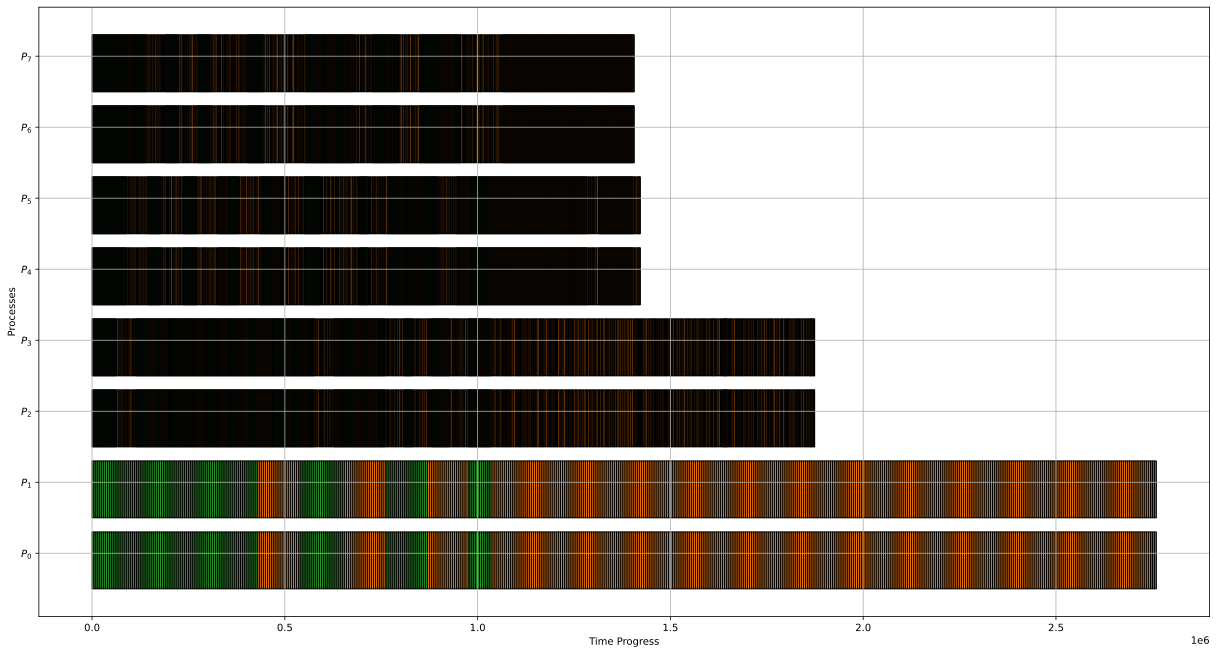
\includegraphics[scale=0.36]{./pictures/perf_analysis_model/perf_model_simulate_react_lb_1000_tasks_per_rank.pdf}
	\caption{An example simulation run with reactive load balancing in the scenario of $8$ processes, $1000$ tasks/process.}
	\label{fig:react_lb_simulation_1000_tasks_per_rank_example}
\end{figure}

Following the time steps and actions simulated for Scenario $1$, the module \texttt{Profiler} of our simulator can record the information, such as when tasks are queued and started execution, migration, termination, to profile the behavior of reactive load balancing. Typically, Figure \ref{fig:react_lb_simulation_1000_tasks_per_rank_example} depicts the profiled task execution over time progress by the simulator. The x-axis indicates time progress, while the y-axis indicates $8$ processes in this simulation scenario. We configure $8000$ tasks in total and $1000$ tasks/process as a given distribution. Process $P_{0}$ and process $P_{1}$ are the slowdown processes. With the given scale of $5 \times$ slower than normal, one task is executed in $5$ seconds. Without load balancing, the total load of process $P_{0}$ and $P_{1}$ would be $5000$s. Through applying reactive load balancing, we can see that the completion time is reduced to around $2700$s.\\

In Figure \ref{fig:react_lb_simulation_1000_tasks_per_rank_example}, a range of ``green'' slots indicates local task execution, while ``orange'' indicates remote task execution. Such an example simulator run, we simply configure the overhead information, consisting of:
\begin{itemize}
	\item Balancing operation overhead (named $O_{\text{balancing}}$): $20$ms occupied $2\%$ of task execution time unit. This means a task is executed in $1$s ($1000$ms), then balancing operations at once take $20$ms. As mentioned in Subsection \ref{subsec:discrete_time_model}, $O_{\text{balancing}}$ accounts for the time of monitoring ($m_{i}(t, t+\Delta t)$) and exchaning load information ($b_{i}(t - \lambda)$).
	\item Task migration overhead (represented by delay time $d$): $10$ms occupied $1\%$ of the task execution time unit.
\end{itemize}

As we can see in Figure \ref{fig:react_lb_simulation_1000_tasks_per_rank_example}, reactive task migration is sometimes incorrect because process $P_{0}$ and $P_{1}$ are known as overloaded processes but they still receive remote tasks. This also happens in a real execution with certain cases of high imbalance alongside many tasks per process and small execution time per task In Figure \ref{fig:react_lb_simulation_1000_tasks_per_rank_example} with the processes $P_{2}$, $...$, $P_{7}$, the area of local tasks is tight and overlaps together; therefore, we might not see clear local task execution. With process $P_{0}$ and $P_{1}$, the area of remote tasks is marked such incorrect task offloading at several time slots.\\

The following subsection provides further details about the evaluation of our simulator. We intend to show the impact between balancing operation overhead and task migration overhead. Notably, we address why reactive load balancing is late at runtime in distributed memory systems.

% We have these constraints to declaring imbalance context based on the number of involved processes ($P$), tasks ($T$), the scale of slowdowns such as $20\%$, $30\%$, or $50\%$, ..., then the number of processes being slow. The last input is the execution rate which denotes how many tasks can be done per time unit, or we can say how the throughput of execution (tasks/time unit) is.\\

% Below the \texttt{Simulation Engine spec.} region is an iteraction region, including \texttt{Balancer} and \texttt{Migrator}. Each time clocking, the balancer will check the queue's status for imbalance ratio ($R_{imb}$). If $R_{imb}$ meets the requirement of offloading tasks, it will signal \texttt{Migrator} for further actions to offloading tasks. Additionally, there is the second interaction region named \texttt{Profiler}. Before a time clock is closed, we can trigger the profiler to trace and record data for visualizing the simulation of our execution with dynamic load balancing. As we can see, the diagram extends the design in Figure \ref{fig:react_lb_simulator} to a communication diagram in more detail. Following the action arrows, we can determine the working flow from the points of simulation view. For example, after getting the imbalance context, we start with \texttt{queue\_setup()}, and \texttt{Clocking} is managed to proceed. Then, the behavior contineou by checking the queues (\texttt{check\_queue()}), ... until the termination of a loop (at \texttt{4.} \texttt{increase} \texttt{\_clock()}).\\

\subsection{Simulator Evaluation}
\label{subsec:Simulator-Evaluation}

\subsubsection{Example without load balancing}
\label{subsubsec:eval-sim-example-no-lb}

The simulation scenario in this subsection is similar to the previous example of Figure \ref{fig:react_lb_simulation_1000_tasks_per_rank_example}. However, we reduce the total number of tasks to reduce simulation time, where each process holds $100$ tasks. The imbalance ratio is also configured $R_{imb} = 1.5$, $P = 8$ processes, and below is an input sample for configuring the simulator.

\begin{lstlisting}[language=Python, caption={Input sample for the baseline simulation.}, label={lst:sim_input_sample}]
	num_process: 8
	num_tasks:   800
	slowdown:    0.2 # the scale of slowdown
	num_sld_processes: 2 # the number of slowed processes
	bandwidth: 1485 MB/s # bandwidth value for calculating delay
	exe_rate: 1.0 task/s # the execution rate
\end{lstlisting}
\hfill

\begin{figure}[t]
  \centering
  \includegraphics[scale=0.65]{./pictures/poc_implementation/poc_visualize_baseline_case_8_processes.pdf}
	\caption{Visualization of the baseline simulation without load balancing.}
	\label{fig:simulator_baseline_case}
\end{figure}

This input is used to simulate the baseline without load balancing. Technically, module \texttt{Balancer} is deactivated in this case. Therefore, there are no values for balancing operation overhead and task migration overhead. With time steps in milliseconds (ms), the clock is counted one by one at a time. In normal processes, the execution rate is $1.0$ task/s, and the total load value of each is ideally $100$s. In slowdown processes, the execution rate is $0.2$, where we simply set process $P_{0}$ and $P_{1}$ as the slow processes. Executing each task in process $P_{0}$ and $P_{1}$ takes $5$s. The completion time without load balancing is $500$s in total. Figure \ref{fig:simulator_baseline_case} shows the simulated baseline. The x- and y-axis also point to the time progress and the load-value bars of $8$ processes. Green boxes denote the executed tasks that are clearly seen at process $P_{0}$ and process $P_{1}$. The load values on other processes are smaller compared to process $P_{0}$ and $P_{1}$ due to many overlapped tasks. Hence, we might see task execution on their sides black (not clearly green as expected).\\

The following is a detailed statistic output from our simulator (Listing \ref{lst:sim_output_sample}). First, the configuration information (under the block \texttt{Configuration}) is summarized. Second, under the block \texttt{Executed Tasks}, the output summarizes the number of local and remote tasks executed on each process. Then, the blocks \texttt{Total Load} and \texttt{Statistic} summarize the total load values of processes and the corresponding maximum, minimum, average load values, resulting in the imbalance ratio. Overall, the detailed output and profiled data can be directed to a \texttt{csv}-format file.

\begin{lstlisting}[language=Python, caption={The output of the baseline simulation.}, label={lst:sim_output_sample}]
-------------------------------------------
Configuration
-------------------------------------------
   + num. processes:     8
   + num. tasks:       800
   + slowdown:         0.2
   + num. sld.procs:     2
   + bandwidth:      1485.0 (MB/s)
   + exe_rate:         1.0 (task/s)
-------------------------------------------

-------------------------------------------
Summary: Executed Tasks
-------------------------------------------
	 + P[0]: num.local_tasks=  100, num.remote_tasks=    0
	 + P[1]: num.local_tasks=  100, num.remote_tasks=    0
	 + P[2]: num.local_tasks=  100, num.remote_tasks=    0
	 + P[3]: num.local_tasks=  100, num.remote_tasks=    0
	 + P[4]: num.local_tasks=  100, num.remote_tasks=    0
	 + P[5]: num.local_tasks=  100, num.remote_tasks=    0
	 + P[6]: num.local_tasks=  100, num.remote_tasks=    0
	 + P[7]: num.local_tasks=  100, num.remote_tasks=    0
-------------------------------------------

-------------------------------------------
Summary: Total Load
-------------------------------------------
   + P[0]: local_load= 500.00(s), remot_load=   0.00(s)
   + P[1]: local_load= 500.00(s), remot_load=   0.00(s)
   + P[2]: local_load= 100.00(s), remot_load=   0.00(s)
   + P[3]: local_load= 100.00(s), remot_load=   0.00(s)
   + P[4]: local_load= 100.00(s), remot_load=   0.00(s)
   + P[5]: local_load= 100.00(s), remot_load=   0.00(s)
   + P[6]: local_load= 100.00(s), remot_load=   0.00(s)
   + P[7]: local_load= 100.00(s), remot_load=   0.00(s)
-------------------------------------------

-------------------------------------------
Statistic
-------------------------------------------
max. load:   500.0
min. load:   100.0
avg. load:   200.0
R_imb:         1.5
sum. overloaded_load:    600.0
sum. underloaded_load:   600.0
-------------------------------------------
Write profiled queue data to: ./poc_visualize_baseline_case_8_procs_output.csv
-------------------------------------------
\end{lstlisting}
\hfill

\subsubsection{Example with reactive load balancing}
\label{subsubsec:eval-sim-example-reactlb}

In the case of applying reactive load balancing, we activate \texttt{Balancer} and configure the values for balancing operation overhead and task migration overhead. With a simulation trial, we initially set the balancing overhead, $O_{\text{balancing}} = 1.0$ms, and delay time, $d=1.0$ms. Compared to the execution time unit of a task in second, we highlight that balancing overhead and delay time occupy $0.1\%$.\\

\begin{figure}[t]
  \centering
  \includegraphics[scale=0.65]{./pictures/poc_implementation/poc_visualize_reactlb_O1_d1_8_processes.pdf}
	\caption{Visualiztion of reactive load balancing case of simulation with $O_{\text{balancing}} = 1.0$ms and $d=1$ms.}
	\label{fig:simulator_reactlb_O1_d1_case}
\end{figure}

Figure \ref{fig:simulator_reactlb_O1_d1_case} shows the visualization of the simulation with reactive load balancing, where $O_{\text{balancing}} = 1.0$ms and $d = 1.0$ms. The x- and y-axis shows time progress and processes executing tasks, where ``green'' and ``orange'' slots indicate local can remote tasks. Overall, the completion time is reduced. The simulated operations of reactive task offloading with $O_{\text{balancing}}$ and $d$ are acted as follows.
\begin{itemize}
	\item Suppose at a time $t_{k}$, module \texttt{Balancer} detects an imbalance and tasks from process $P_{0}$ are then offloaded to process $P_{7}$ as an example. However, the tasks are proceeded in the queue for offloading at time $t_{k} + 1$ because of $O_{\text{balancing}} = 1.0$.
	\item Similarly, assuming tasks from process $P_{0}$ are decided to offload to process $P_{7}$ at $t_{k}$. However, these tasks arrive at process $P_{7}$ at time $t_{k} + 1$ because of $d = 1.0$.
\end{itemize}

In the simulator, module \texttt{Clocking} controls the ticking procedure of time steps. We can adjust this procedure to simulate the execution of dynamic load balancing similar to running in practice. Listing \ref{lst:sim_output_reactlb_O1_d1} shows the output sample of this simulated scenario. The output format is equivalent to Listing \ref{lst:sim_output_sample}, but we skip the part of \texttt{Configuration}. As a result, the summary under block \texttt{Executed Tasks} highlights the number of remote tasks from process $P_{2}$ to $P_{7}$. In response to the number of remote tasks, block \texttt{Total Load} indicates the total load values of remote tasks, proving that reactive load balancing works. In the end, the completion time is improved significantly $\approx 165.0$ms, and $R_{imb}$ is almost $0.0$.

\begin{lstlisting}[language=Python, caption={The simulation output of reactive load balancing with $O_{\text{balancing}} = 1.0$ms, $d=1$ms}, label={lst:sim_output_reactlb_O1_d1}]
-------------------------------------------
Configuration
-------------------------------------------
   ...
-------------------------------------------

-------------------------------------------
Summary: Executed Tasks
-------------------------------------------
	 + P[0]: num.local_tasks=   33, num.remote_tasks=    0
	 + P[1]: num.local_tasks=   33, num.remote_tasks=    0
	 + P[2]: num.local_tasks=   82, num.remote_tasks=   38
	 + P[3]: num.local_tasks=   82, num.remote_tasks=   38
	 + P[4]: num.local_tasks=   81, num.remote_tasks=   42
	 + P[5]: num.local_tasks=   81, num.remote_tasks=   42
	 + P[6]: num.local_tasks=   76, num.remote_tasks=   48
	 + P[7]: num.local_tasks=   76, num.remote_tasks=   48
-------------------------------------------
	
-------------------------------------------
Summary: Total Load
-------------------------------------------
   + P[0]: local_load= 165.00(s), remot_load=   0.00(s)
   + P[1]: local_load= 165.00(s), remot_load=   0.00(s)
   + P[2]: local_load=  82.00(s), remot_load=  72.50(s)
   + P[3]: local_load=  82.00(s), remot_load=  72.50(s)
   + P[4]: local_load=  81.00(s), remot_load=  75.00(s)
   + P[5]: local_load=  81.00(s), remot_load=  75.00(s)
   + P[6]: local_load=  76.00(s), remot_load=  81.00(s)
   + P[7]: local_load=  76.00(s), remot_load=  81.00(s)
-------------------------------------------

-------------------------------------------
Statistic:
-------------------------------------------
max. load:   165.0
min. load:   154.5
avg. load:   158.1
R_imb:         0.0
sum. overloaded_load:     13.8
sum. underloaded_load:    13.8
-------------------------------------------
Write profiled queue data to: ./profiled_queues_reactlb_O1_d1.csv
-------------------------------------------
\end{lstlisting}

\subsubsection{Experiments with the simulator}
\label{subsubsec:eval-sim-experiments-reactlb}

\begin{figure}[t]
\centering
\subfloat[Subfigure1][Reactive LB with $O_{\text{balancing}}$ $=2$ms and $d=2$ms]{
\includegraphics[scale=0.525]{./pictures/poc_implementation/poc_visualize_reactlb_O2_d2_8_processes.pdf}
\label{sfig:reactlb_O2_d2}}
\subfloat[Subfigure2][Reactive LB with $O_{\text{balancing}}$ $=5$ms and $d=2$ms]{
\includegraphics[scale=0.525]{./pictures/poc_implementation/poc_visualize_reactlb_O5_d2_8_processes.pdf}
\label{sfig:reactlb_O5_d2}}
\qquad
\subfloat[Subfigure3][Reactive LB with $O_{\text{balancing}}$ $=10$ms and $d=2$ms]{
\includegraphics[scale=0.525]{./pictures/poc_implementation/poc_visualize_reactlb_O10_d2_8_processes.pdf}
\label{sfig:reactlb_O10_d2}}
\subfloat[Subfigure4][Reactive LB with $O_{\text{balancing}}$ $=20$ms and $d=2$ms]{
\includegraphics[scale=0.525]{./pictures/poc_implementation/poc_visualize_reactlb_O20_d2_8_processes.pdf}
\label{sfig:reactlb_O20_d2}}
\caption{A visualization of reactive load balancing with increased balancing overhead and delay.}
\label{fig:simulator_reactlb_increased_Ovaried_d2}
\end{figure}

To see the effects of balancing overhead, we try to increase $O_{\text{balancing}}$ first from $2$, $5$, $10$, to $20$ms, corresponding to the occupation of $0.2\%$, $0.5\%$, $1.0\%$, $2.0\%$ over task execution time unit, while $d = 2$ is kept constantly. Figure \ref{fig:simulator_reactlb_increased_Ovaried_d2} shows these tests in the visualization of reactive load balancing (denoted by Reactive LB). Compared to the baseline (in Figure \ref{fig:simulator_baseline_case} on Page \pageref{fig:simulator_baseline_case}) and the initial imbalance scenario (in Figure \ref{fig:simulator_reactlb_O1_d1_case} on Page \pageref{fig:simulator_reactlb_O1_d1_case} with $O_{\text{balancing}}$ $=1$ms, $d=1$ms), Figure \ref{fig:simulator_reactlb_increased_Ovaried_d2} highlights the impact of balancing operation overhead. Not only delay time, load balancing operations in monitoring, exchanging load information/queue status, and calculating imbalance conditions can also significantly affect overall performance. $O_{\text{balancing}}$ is sensitive when almost all dynamic load balancing methods decide on many continuous actions and task migrations. For instance, the balancing decisions start getting worse when $O_{\text{balancing}}$ occupies $0.5\%$ over task execution time unit.\\

\begin{figure}[t]
\centering
\subfloat[Subfigure1][Reactive LB in that keep $O_{\text{balancing}}=2$ constantly and vary $d$]{
\includegraphics[scale=0.4]{./pictures/perf_analysis_model/perf_model_queue_decrease_delay_impact_OB2.pdf}
\label{sfig:reactlb_O2_dvaried}} \\

\subfloat[Subfigure2][Reactive LB in that keep $O_{\text{balancing}}=5$ constantly and vary $d$]{
\includegraphics[scale=0.4]{./pictures/perf_analysis_model/perf_model_queue_decrease_delay_impact_OB5.pdf}
\label{sfig:reactlb_O5_dvaried}} \\

\subfloat[Subfigure3][Reactive LB in that vary $O_{\text{balancing}}$ and keep $d=2$ constantly]{
\includegraphics[scale=0.4]{./pictures/perf_analysis_model/perf_model_queue_decrease_blancing_impact_d2.pdf}
\label{sfig:reactlb_Ovaried_d2}}

\caption{Evaluation of the queue length convergence when varying task migration overhead (delay) and balancing operation overhead.}
\label{fig:evaluation_Obalancing_effects}
\end{figure}

For another evaluation, we keep $O_{\text{balancing}}$ as a constant and vary $d$ to see the impact of task migration overhead, Figure \ref{fig:evaluation_Obalancing_effects} shows two experiments conducted, one in Figure \ref{sfig:reactlb_O2_dvaried} showing $O_{\text{balancing}}=2$ and $d$ is ranged from $0.1\%$ to $2\%$; one in Figure \ref{sfig:reactlb_O5_dvaried} showing $O_{\text{balancing}}=5$ and $d$ is ranged from $0.1\%$ to $2\%$. The imbalance scenario is stayed similar to the previous tests. In both figures, the x-axis indicates the progress of queues changed over time steps (in ms); the y-axis indicates the queue length as the number of remaining tasks over time steps.\\

Generally, all the queues are converged into $0$ at the end after the execution is finished. However, the slope of different queue lines might be different because some processes are slowed down and execute tasks slower. Note that these experiments with the simulator are applied reactive load balancing, and the final results show the load balancing performance. Typically, the slope in these figures represents how efficient the performance is. The last queue converged at shorter time steps determines a better performance. The balancing operation overhead is still trivial with $O_{\text{balancing}}=2$. We can see that increasing $d$ does not affect the convergence speed much. However, with $O_{\text{balancing}}=5$, delay $d$ here is more sensitive, and the convergence of queues gets impacted. Following this, if we compare with the experiments visualized in Figure \ref{fig:simulator_reactlb_increased_Ovaried_d2} (on Page \pageref{fig:simulator_reactlb_increased_Ovaried_d2}) when $d$ is constant and $O_{\text{balancing}}$ is varied, Figure \ref{sfig:reactlb_Ovaried_d2} emphasizes in detail these scenarios with the convergence of queue lengths. For a slightly change of $O_{\text{balancing}}$, the load balancing performance is significantly affected.



\section{Towards Proactive Idea in Dynamic Load Balancing and Co-scheduling Tasks}
\label{sec:Idea-Proactive-LB}
\index{PerfModel!A Proactive Idea for Load Balancing}

The previous section highlights that task migration overhead in distributed memory systems is not the only primary influence factor. Instead, balancing operation overhead can also affect our performance. The balancing operations consist of monitoring queue information or status, calculating imbalance, exchanging status information, and making decisions on task migration. The overhead of each operation might be small and trivial. However, when they are performed numerously and continuously, the decisions of task migration can be significantly impacted. Eventually, the performance of load balancing is affected overall.\\

This subsection emphasizes three representative pillars that lead to wrong decision-making for reactive load balancing in particular and dynamic load balancing in general. Figure \ref{fig:three_pillars_reactlb} shows these pillars from left to right, including:
\begin{itemize}
	\item The first pillar implies the factors of imbalance reason (in our context, slowdown is mentioned and denoted by $S_{P}$) and imbalance level ($R_{imb}$).
	\item The second pillar is related to the overhead of load monitoring ($m$) and information exchanging ($b$).
	\item The third pillar is the overhead of task offloading, indicating the delay time ($d$) when tasks are migrated.
\end{itemize}

\begin{figure}[t]
  \centering
  \includegraphics[scale=0.55]{./pictures/perf_analysis_model/perf_three_pillars_of_react_lb.pdf}
	\caption{Three pillars of factors might challenge reactive load balancing.}
	\label{fig:three_pillars_reactlb}
\end{figure}

Concretely, the first pillar implies imbalance context related to performance slowdown, leading to high or low imbalance levels. The second pillar is overhead in the middle, revolving around balancing operations. At runtime, all dynamic load balancing methods perform seemingly random operations before a task can be migrated. The last pillar is about overhead and decision-making for task offloading as well as task migration. If the second pillar takes a small overhead, then decisions in the third pillar can be made faster. When tasks are decided to migrate, the main overhead is delay time $d$, which $d$ is large or small, depending on the data size of tasks, latency, and network bandwidth. We describe the interaction between these pillars as follows.
\begin{itemize}
	\item If $R_{imb}$ is high, the imbalance condition might be detected in high frequency. Then, task offloading decisions are made many times.
	\item To know how many tasks and where to offload tasks, there are different ways to make decisions associated with the first pillar.
	\begin{itemize}
		\item For safety, exactly one task should be moved at one point in time. However, this might lead to many monitoring, checking, and exchanging load information operations. Simultaneously, the big enough values of $d$ can make these points challenging because it can take time to finish the exchanging operations before a task is decided for migration.
		\item To reduce the number of migration procedures, several tasks can be moved at once. However, deciding how many tasks are appropriate without prior knowledge is difficult.
	\end{itemize}
\end{itemize}

We can see that ``reactive'' load balancing implies taking actions reactively based on the most current status. This also means that we cannot plan to decide how many tasks should be migrated at a time adaptively. Besides, there is no information about which process could be a potential victim. When balancing operation and task migration produce a certain overhead, the decisions of reactive load balancing can be late and incorrect.\\

In general, we highlight that the challenge of dynamic load balancing is to obtain prior knowledge about load information. Assuming that we can predict load information or generate knowledge about load information at runtime, we can drive load balancing better. This thesis motivates an idea: How can we perform load balancing more proactively at runtime? ``Proactive'' implies that we can calculate how bad the imbalance is at a current state and how many tasks should be migrated at once. Consequently, we propose a proactive load balancing approach that enables to characterize task execution, learn load information, and predict imbalance. This is considered a better prognostication compared to the reactive load balancing approach. From idea to practice, our proactive approach is developed by the following technical questions:
\begin{itemize}
	\item Can we use a dedicated thread to obtain load values at runtime?
	\item Can we leverage the profiled information of several first iterations (or previous iterations) to generate the load knowledge?
	\item Can we change from reactive to more proactive task offloading between iterations?
\end{itemize}

For most of the use cases in HPC, iterative applications or simulation frameworks can benefit from our approach. Their behaviors are divided into multiple execution phases (so-called iterations). With a large simulation use case, a program can be run with many iterations, and an adaptive approach for load balancing is essential. Therefore, our proactive idea can be relevant to make load balancing more adaptive. The following chapter will show in detail how we design the idea.

% Taking a look at the condition for task offloading, it relies on setting an imbalance threshold and the availability of tasks at a time.

%\section{Related Models for Work Stealing}
\label{sec:Refer-Model-WS}
\index{PerfModel!Related Models for Work Stealing}

\begin{figure}[t]
  \centering
  \includegraphics[scale=0.8]{./pictures/perf_analysis_model/perf_analysis_related_model_without_latency.pdf}
	\caption{An illustration of work-stealing without latency concern.}
	\label{fig:perfmodel_relatedmodelwithoutlatency}
\end{figure}

As mentioned, we illustrate again an example of work stealing behaviors in Figure \ref{fig:perfmodel_relatedmodelwithoutlatency}, but this case is without latency concern. This model is commonly known in shared memory systems. The idea is that idle processes will try to steal tasks from other busy processes. Communication is assumed very fast to send and receive tasks immediately. As we can see, the x-axis shows the execution progress by time, along with four processes indexed from 0 to 3. The triangles represent stealing operations at a time. This is an ideal case for load balancing when the time to send and receive tasks is almost instantaneous.\\

To demystify the related models and our proposed model in the next sections, we attempt to merge some related terminologies as well as notations so that they are consistent in this thesis. For example, the total number of tasks is reused and named $T$, distributed on $P$ processes before execution. Table \ref{tab:mapped_notation_table} will show in detail the other related notations. Such the concern, each process in $P$ after a given distribution of $T$ tasks will hold a subset of $T_{i}$ tasks. In some related works, they used $w_{i}$ to indicate the number of tasks at process $i$  \cite{tchiboukdjian2013decentralized}. Thereby, we try to make it consistent with us by using $T_{i}$ as the number of tasks in process $i$. In the following sections, there might be some additional terms about the queue information, and $Q_{i}$ is used to denote the queue status, and they still refer to the values of the number of tasks. Mapping them to the time progress, this may have the field of time $(t)$ following. For instance, $T_{i}(t)$ means the number of tasks in process $i$ at time $t$, or $T(t)$ without $i$ means the total number of tasks (including all processes) at time $t$. The text might re-mention these notations in some specific paragraphs when we want to show further explanation.\\

\begin{table}[t]
\centering
\begin{tabular}{|l|p{2cm}|p{5cm}|p{4.5cm}|}
\hline
\textbf{No.} & \textbf{Notations} & \textbf{Description} & \textbf{Note}        \\ \hline
1  & $T$          & the number of tasks indexed $\left \{0,...,(T-1) \right \}$ & In some other related works, people used $W$ instead of $T$   \\ \hline
2  & $P$					& the number of processes, $\left \{0,...,(P-1) \right \}$    & Other works might use $m$ identical processors instead of $P$ \\ \hline
3  & $T_{i}$			& the set of assigned tasks in Process $i$                    & Other works might use $w_{i}$ instead of $T_{i}$              \\ \hline
4  & $L_{i}$			& the total load of Process $i$                               &                                             \\ \hline
5  & $w_{i}$			& the wallclock execution time of a task, i.e., task $i$      &                                             \\ \hline
6  & $W_{i}$ 			& the wallclock execution time of Process $i$                 &                                             \\ \hline
7  & $S_{P_{i}}$	& processing speed (performance model) of Process $i$         &                                             \\ \hline
8  & $Slow_{i}$		& slowdown coefficient of Process $i$ at runtime              &                                             \\ \hline
9  & $W_{par}$		& the total wallclock execution time (makespan)               & Also called completion time ($C$)           \\ \hline
10 & $R_{imb}$		& imbalance ratio                                             &                                             \\ \hline
11 & $\lambda$		& communication or network latency                            &                                             \\ \hline
12 & $d$					& delay or transmission time                                  &                                             \\ \hline
13 & $B$					& network bandwidth                                           &                                             \\ \hline
14 & $O_{ij}(t)$	& the number of offloaded tasks from Process $i$ to $j$       & The authors in \cite{tchiboukdjian2010tighter} used $R(t)$ as the number of task requests in global after time $t$ \\ \hline
\end{tabular}
\caption{Used notations in the thesis comparing to the notations from related works.}
\label{tab:mapped_notation_table}
\end{table}

The main purpose of performance modeling is to show an upper bound of balancing efficiency with how many tasks can be migrated. Extended from an original work \cite{Blumofe1999OriginWS}, Tchiboukdjian et al. have proposed a good model for work-stealing without latency since 2010 \cite{tchiboukdjian2010tighter} \cite{tchiboukdjian2013decentralized}. In this section, we attempt to summarize their reference models. The first is mentioned as work stealing model without communication latency \cite{tchiboukdjian2010tighter} \cite{tchiboukdjian2013decentralized}. The second is timely analyzed by \cite{gast2021analysis} in 2021, also work stealing but with latency variable.\\

In \cite{tchiboukdjian2013decentralized}, Tchiboukdjian et al. considered a parallel platform with $P$ processes. At time $t$, $T_{i}(t)$ represents the amount of works\footnote{At this point, works are considered as tasks in our context. Therefore, they might be used interchangeably.} on process $i$. Compared to $t=0$, $T_{i}(t)$ will be decreased by time progress. For example, at $t=0$ the workload is just distributed on each process, $T_{i}(t_{0}) = 100$ means holding 100 tasks before running. Then, at $t=10$ assume that 10 tasks have been done on process $i$, and $T_{i}(t_{10})$ would be $90$ such the remaining tasks. We can take Figure \ref{fig:perfmodel_relatedmodelwithoutlatency} as an example, at $t=10$ process $3$ has done 10 tasks and its queue remains 90 tasks, $T_{0}(t_{10}) = 90$. In constract, process $2$ is faster and it has done all tasks at $t=10$, therefore, $T_{2}(t_{10}) = 0$.\\

Therefore, the execution behavior will be simplified as follows,
\begin{itemize}
	\item when $T_{i}(t) > 0$, processor $i$ is active and execute tasks, $T_{i}(t+1) \leq T_{i}(t)$.
	\item when $T_{i}(t) = 0$, processor $i$ is idle and intends to steal tasks from a random processor $j$.
\end{itemize}

\noindent \textbf{A Tight Analysis of Work Stealing \cite{tchiboukdjian2010tighter,tchiboukdjian2013decentralized}}\\

If work stealing is applied, some tasks are moved around, then $T_{i}(t)$ will increase or decrease, depending on how many steal requests and tasks are performed at a time. Tchiboukdjian et al. \cite{tchiboukdjian2010tighter} \cite{tchiboukdjian2013decentralized} assumed that between time $t$ and $t+1$, there are $P - \alpha(t)$ steal requests, $P$ is the total number of processes and $\alpha(t)$ denotes the number of active processes, $\alpha(t) \in [0, m]$. When $\alpha(t)=0$, it means all queues are empty as well as the execution is complete. Corresponding to the sucess steal requests, process $j$ will transfer an amount of work to $i$ and $T_{i}(t+1) + T_{j}(t+1) \leq T_{j}(t)$. Similar to when $\alpha(t)=0$, the execution will terminate if $\forall i \in P, T_{i}(t) = 0$. At time $t$, the total number of tasks on all processes is denoted by $T(t) = \sum_{i=1}^{P}T_{i}(t)$. After that, process $2$ will steal some tasks from the others to help share the load. The triangle shows stealing operations, and there is obviously stealing overhead in practice. However, we show this related model with an assumption about no latency, in which the use cases might be considered in shared memory.\\

In the baseline without work-stealing, the total execution time depends on the process with a maximum load, $C_{max} = max_{i \in P} T_i(t_0)$, so-called makespan or critical path. When we use work stealing, $C_{max}$ can be reduced. Therefore, the main question of work stealing model is:
\begin{shaded}
	\noindent What is the upper bound of makespan when work stealing is applied?
\end{shaded}

The work has proposed a potential function $\Phi (t)$ to model the performance of work stealing through studying the potential decrease. Assuming that tasks are unit independent, $\Phi (t)$ is defined by
\begin{equation} \label{eq:phi_defi}
	\Phi(t) = \sum_{i=1}^{P} (T_{i}(t) - \frac{T(t)}{P})^{2} = \sum_{i=1}^{P} T_{i}(t)^{2} - \frac{T(t)^2}{P}
\end{equation}
where, the potential represents the load unbalance of execution. For example, as expected at time $t$ the average load among $P$ processes is $\frac{T(t)}{P}$. Then, if we sum the difference values between each process's load value at $t$ and the average value, the result shows how much load difference is. \\

Therefore, the decrease of $\Phi (t)$ depends on the number of steal requests and execution scenario. The above has mentioned an estimated formular for the number of steal requests ($P - \alpha(t)$). $\alpha(t)$ is a complicated random process that chooses the number of active processors at each step. Such an expectation in work-stealing, the more work requests it creates, the more the potential will decrease. The performance analysis model is performed in three steps:
\begin{enumerate}
	\item Define $\Phi (t)$.
	\item Compute the expected decrease of $\Phi (t)$ between step $t$ and $t+1$, $\Delta \Phi (t) \overset{def}{=} \Phi (t) - \Phi (t+1)$. However, at a specific time $t$, how can we estimate the decrease? To this end, the authors define another term, named $\delta_{i}^{k}(t)$, to compute the expected decrease,
	\begin{equation} \label{eq:expect_decrease}
		\sum_{i=1}^{P} \sum_{k=0}^{P-1} E [\delta_{i}^{k}|i\ \textrm{receives}\ k\ \textrm{requests}]P\left \{ i\ \textrm{receives}\ k\ \textrm{requests} \right \}
	\end{equation}
	
	, where the first sum goes through all $P$ processes and the second sum goes from $0$ to $(P-2)$ as the maximum requests a process can get at a time. $E[X|Y]$ denotes the expectation of $X$ knowing $Y$. Applying this to the example in Figure \ref{fig:perfmodel_relatedmodelwithlatency} we have
	
	\begin{equation}
		E[\Delta \Phi (t)] = \sum_{i=0}^{3} \sum_{k=0}^{3} E [\delta_{i}^{k}|i\ \textrm{receives}\ k\ \textrm{requests}]P\left \{ i\ \textrm{receives}\ k \textrm{requests} \right \}
	\end{equation}

	Following that, the authors showed that there exists a function called $h(\alpha) \in (0;1]$ such that $E[\Delta \Phi (t)|\Phi (t) = \Phi,\alpha(t) = \alpha] \geq h(\alpha) \Phi$.
	
	\item This work obtained a bound on the expected number of steal requests $E[R]$ ($R$ is the number of steal requests), and the expected makespan $E[C_{max}]$ can be further obtained from $E[R]$.
\end{enumerate}

This work concluded that the expected number of steal requests $R$ until $\Phi(t) \leq 1$ is bounded by $E[R] \leq \lambda \cdot P \cdot log_{2} \Phi(0)$, where $\lambda$ in this case is $max_{1 \leq \alpha \leq P-1} \frac{P-\alpha}{-P \cdot log_{2}(1-h(\alpha))}$ and $\Phi(0)$ is the potential at $t=0$. At the end, the expected value of $C_{max}$ will be bounded by 
\begin{equation}
	E[C_{max}] \leq \frac{T}{P} + \frac{2}{1-\log_{2}(1+\frac{1}{\epsilon})} \log_{2}W + 1
\end{equation}

Before \cite{tchiboukdjian2010tighter,tchiboukdjian2013decentralized}, some previous works also attempted to find an upper bound. One of the original studies from Blumofe and Leiserson \cite{Blumofe1999OriginWS} showed that the efficiency of work-stealing is bounded by $E(C_{max}) \leq \frac{T}{P} + O(D)$, where $D$ is the length of the critical path in the case of dependent tasks (represented as a graph). The analysis is further improved by \cite{arora2001thread} using potential functions. The authors used an amortization argument based on a potential function that decreases as the work-stealing algorithm processes. The idea is to divide the execution into phases and show that the potential decreases by at least a constant fraction with a constant probability. For the case of varying the speed of $P$ processors or heterogeneous processors, Bender and Rabin \cite{bender2002online} provided a new analysis of an old scheduling algorithm called \textit{maximum utilization scheduler}. The authors showed a given context for $P$ processors with speed $\pi_{i}$ steps/time. These studies are constrained in a context of only one source of tasks that could not easily model the basic case of independent tasks, and communication overhead is not explicitly counted.\\

\noindent \textbf{A Tighter Analysis of Work Stealing with Latency \cite{gast2021analysis}} \\

For modeling with communication latency, people are rarely concerned explicitly in work-stealing models. In 2021, Nicolas Gast et al. \cite{gast2021analysis} proposed a new analysis model on how communication latency impacts stealing operations in terms of task-parallel applications. The model has been created for distributed memory clusters with $P$ identical processors. Latency value is denoted by $\lambda$. The authors inherited from their previous work \cite{tchiboukdjian2013decentralized} and aimed at an upper bound for the expected makespan.\\

We investigate this related work in more detail which motivates us to propose a new model. From one of the previous studies \cite{tchiboukdjian2013decentralized}, the authors also make a consistent assumption about work-stealing algorithms in general:
\begin{itemize}
	\item The total number of processes is defined as $P$ identical processors.
	\item $T_{i}(t)$ denotes the amount of tasks on processor $i$ at time $t$, and the total tasks at $t$ would be $T(t) = \sum_{i=1}^{P}T_{i}(t)$. 
	\item A task corresponds to one unit of execution time.
	\item Latency: all communication take $\lambda \in N$ time unit.
	\item Single Task Transfer: a processor can send some tasks to at most one processor at a time.
	\item Steal Threshold: if the victim has less than $\lambda$ task units to execute, the stealing request will be failed.
	\item Task to be stolen: the victim sends to the thief half of its tasks at a time. For example, the total tasks of process $i$ at time $t$ is $T_{i}(t) = \frac{T_{i}(t-1) - 1}{2}$.
\end{itemize}

\begin{figure}[t]
  \centering
  \includegraphics[scale=0.8]{./pictures/perf_analysis_model/perf_analysis_related_model_with_latency.pdf}
	\caption{An illustration of work-stealing with latency effect.}
	\label{fig:perfmodel_relatedmodelwithlatency}
\end{figure}

Figure \ref{fig:perfmodel_relatedmodelwithlatency} demonstrates a scenario of work stealing with latency. The x-axis represents the time progress of execution with four involved processes. Process $2$ is assumed idle and sends a steal request to process $3$. Since process $3$ accepts, task is sent from $3$ to $2$. We name $\lambda$ as the latency, and one stealing action takes a round-trip time $2\lambda$. This occurs similarly between process $1$ and $0$.\\

As the round-trip time of $2\lambda$ and the total amount of tasks $T$ on $P$ processes, we can drive to a straightforward bound of makespan as \ref{eq:straight_cmax}.
\begin{equation} \label{eq:straight_cmax}
\begin{split}
	P \cdot & C_{max} \leq T + 2\lambda \cdot \#{\textrm{task requests}} \\
	\Leftrightarrow \ & C_{max} \leq \frac{T}{P} + 2\lambda \cdot \frac{\#{\textrm{task requests}}}{P}
\end{split}
\end{equation}

However, to be closer to an optimal bound, this work approached a potential function bounding on the number of work-stealing requests\footnote{Work-stealing requests mean the number of requests for stealing tasks in our context. Therefore, it is also called $\#{\textrm{task requests}}$ shown in Equation \ref{eq:straight_cmax} or steal requests}. The authors reconsidered the time division as periods of duration $\lambda$ to analyze the impact of latency. To not abuse notations, we use $T_{i}(k)$ and $s_{i}(k)$ to denote the current number of tasks and the number of stolen tasks from process $i$ at time $k$; then the quantities will be $T_{i}(k\lambda)$, $s_{i}(k\lambda)$. In the interval $(\lambda (k-1), \lambda k]$, the total number of incoming work-stealing requests is defined by $r(k) = \sum_{i=1}^{\lambda} R((k-1)\lambda + i)$, where $0 \leq r(k) \geq P$. The probability, that a process receives $\geq 1$ requests in the interval $(\lambda (k-1), \lambda k]$, is $q(r(k))$.\\

Nicolas Gast et al. \cite{gast2021analysis} showed the analysis of the potential decrease, which is defined in Equation \ref{eq:potfunc_latency} at time-step $k\lambda$.
\begin{equation} \label{eq:potfunc_latency}
\begin{split}
	\Phi(k) = 1 + \frac{1}{\lambda^2} \sum_{i=1}^{P} (T_{i}(k)^2 + 2s_{i}(k)^2)
\end{split}
\end{equation}

where, $\Phi(k)$ gets through all processes $\in P$, $T_{i}(k)$ and $s_{i}(k)$ represents the number of remaining tasks as well as the number of stolen tasks in process $i$ at time $k$. Let $\Phi(0)$ be the potential at time $t_{0}$ and $\tau$ be the first time step at which the potential reaches $1$. Then, the authors proved that the number of incoming steal requests until $\tau$, $R = \sum_{k=0}^{\tau = 1} r(k)$ satisfies:
\begin{equation} \label{eq:exp_prob_R_latency}
\begin{split}
	& E[R] \leq P \gamma \log_{2} \Phi(0) \\
	& \mathbb{P}[R \leq P \gamma (\log_{2} \Phi(0) + x)] \leq 2^{-x}
\end{split}
\end{equation}

In which, $E[R]$ is the expected number of total incoming steal requests and $\mathbb{P}$ indicates the probability when $R \leq P \gamma (\log_{2} \Phi(0) + x)$, and $\gamma$ is a constant such that $\gamma < 4.03$. Applying to $C_{max}$, the study concluded as Equation \ref{eq:exp_prob_Cmax_latency} shows.

\begin{equation} \label{eq:exp_prob_Cmax_latency}
\begin{split}
	& E[C_{max}] \leq \frac{T}{P} + 4\lambda\gamma\log_{2} \frac{P}{\lambda} + 2\lambda\gamma \\
	& \mathbb{P}[C_{max} \geq \frac{T}{P} + 4\lambda\gamma\log_{2} \frac{P}{\lambda} + x] \leq 2^{\frac{-x}{2\lambda\gamma}}
\end{split}
\end{equation}


\paragraph{Further discussion:}
The mentioned models above are relevant in terms of work stealing with or without latency. However, latency $\lambda$ is a constant, and the number of steal requests must contribute relatively, such as task execution time. These constraints might be limited by the cases in that task data sizes are different or transmission time considerably impacts the efficiency of stealing operations in practice. In contrast, this thesis analyzes the performance in a different direction. We introduce a proposed model associated with transmission time or delay time. The delay happens when tasks are migrated in distributed memory. First, the delay values depend on the size of task data in movement and the current status of interconnection, e.g., latency, bandwidth. Second, we figure out that this challenge can lead to other impacts on the decision time of taking stealing or balancing actions. This is a reason causing too late to balancing load in distributed memory. Next, we will discuss about a proposed model with delay time when tasks are migrated.


%\section{Model Evaluation}
\label{sec:Model-Evaluation}
\index{PerfModel!Model Evaluation}

This section introduces the experiments with our simulator to show when reactive load balancing can be late sometimes, leading to late decisions in offloading tasks. Our evaluation metric for this case is the decrease in queue length. Each process, in general, has a global queue of tasks. The execution threads per process get tasks from the queue for execution. Therefore, the queue length will be decreased toward $0$ over time steps, where the slowest process with queue length converging to $0$ determines the completion time of our application.\\

To be again consistent with the addressed example in the previous sections, we configure the simulation with $8$ ranks. Each rank here keeps $100$ tasks\footnote{To get the simulation results faster, we have reduced the number of tasks to $100$, compared to the one of $1000$ tasks in Figure \ref{fig:react_lb_simulation_1000_tasks_per_rank_example}.} at the beginning. Two of $8$ ranks are $5\times$ slower than normal, and the normal execution rate is $1$ tasks/second. This means the two slowdown ranks take $5$s to complete a task, while the others take $1$s for a task. In case of no load balancing, the completion time is $500$s because the two bottleneck ranks take $5$s/task. $R_{imb}$ is about $1.5$, clock timing is counted in one-by-one step, in which each step is $1$ms. Alongside, there are two variables varied in the experiments:
\begin{itemize}
	\item Balancing overhead ($O_{\text{balancing}}$): the values are varied such as $1, 2, 5, ...$, accounting for $0.1\%$, $0.2\%$, $0.5\%$ of overhead. 
	\item Delay time in task migration ($d$): its values are also varied such as $1, 2, 5, ...$, and also accounting for $0.1\%$, $0.2\%$, $0.5\%$ of overhead. 
\end{itemize}

\noindent \textbf{Vary delay ($d$) and keep balancing overhead ($O_{\text{balancing}}$) stable}\\
\noindent In this set of simulations, we vary the values of $d$ in a range of $[$ $0.1\%$, $0.2\%$, $0.5\%$, $1\%$, $2\%$ $]$, and keep the values of $O_{\text{balancing}}$ as a constant. \\

\begin{figure}[t]
  \centering
  \includegraphics[scale=0.45]{./pictures/perf_analysis_model/perf_model_queue_decrease_delay_impact_OB2.pdf}
	\caption{A simulation case to show the impact of delay time ($d$) with keeping the overhead of balancing operations as a constant of $0.2\%$.}
	\label{fig:react_lb_sim_delay_impact_Obal_2}
\end{figure}

Figure \ref{fig:react_lb_sim_delay_impact_Obal_2} shows a simulation experiment with the varied values of delay ($d$), while we keep the value of balancing overhead as a constant of $0.2\%$. Note that the percentage means the ratio with task runtime unit. Here the runtime is in seconds, and the values of $d$ or $O_{\text{balancing}}$ are in milliseconds. Therefore, $O_{\text{balancing}}$, in this case, takes $2$ms, occupying $0.2\%$ of a task runtime unit. As the figure shows, there are $8$ processes, where each line indicates the decrease or the convergence of its queue to $0$ over the execution time progress (on the x-axis). The y-axis shows the queue length values. At the very beginning, the queue length of all processes is the same, $100$ tasks. Following execution and reactive load balancing, they tend to decrease steadily but might sometimes increase if receiving tasks from a remote process. There are five plots from left to right, illustrating the simulation when $d$ is varied from $0.1\%$ to $2\%$. The time that the last process goes to $0$ also highlights the completion time. Figure \ref{fig:react_lb_sim_delay_impact_Obal_2} shows that the increasing values of $d$ do not highly change the completion time in this case. Such a baseline, if we do not apply any load balancing methods, the completion time will be $500k$. Therefore, the simulating case in Figure \ref{fig:react_lb_sim_delay_impact_Obal_2} shows that reactive load balancing is significantly useful.\\

\begin{figure}[t]
  \centering
  \includegraphics[scale=0.45]{./pictures/perf_analysis_model/perf_model_queue_decrease_delay_impact_OB5.pdf}
	\caption{A simulation case to show the impact of delay time ($d$) with keeping the overhead of balancing operations as a constant of $0.5\%$.}
	\label{fig:react_lb_sim_delay_impact_Obal_5}
\end{figure}

Next, we try to increase the balancing overhead a little more by $0.5\%$. Figure \ref{fig:react_lb_sim_delay_impact_Obal_5} shows the simulations with $O_{\text{balancing}}=5$. Some queues initially receive tasks from $P0$ and $P1$, for example, $P7$. This is why the $P7$ queue length is larger than $100$ tasks at that moment. In the end, the completion time is still slightly improved ($< 500$k ms) rather than the baseline. However, this simulating case shows that the overhead of balancing operations can greatly impact the time when task offloading is decided to take action. Even though the strategy of reactive load balancing can perform task migration earlier, it is still challenging during decision-making. In the next simulation scenarios, we keep $d$ as a constant and vary the value of $O_{\text{balancing}}$.\\

\noindent \textbf{Vary balancing overhead ($O_{\text{balancing}}$) and keep delay ($d$) stable}\\
\noindent In this set of simulations, we vary the values of $O_{\text{balancing}}$ in a range of $[$ $0.1\%$, $0.2\%$, $0.5\%$, $1\%$, $2\%$ $]$, and keep the values of $d$ as a constant.\\

\begin{figure}[t]
  \centering
  \includegraphics[scale=0.45]{./pictures/perf_analysis_model/perf_model_queue_decrease_blancing_impact_d2.pdf}
	\caption{A simulation case to show the impact of balancing-operations overhead ($O_{\text{balancing}}$) with keeping the delay time as a constant of $0.2\%$.}
	\label{fig:react_lb_sim_Obalancing_impact_d_2}
\end{figure}

Figure \ref{fig:react_lb_sim_Obalancing_impact_d_2} shows the simulation experiments with the varied values of $O_{\text{balancing}}$, while we keep $d$ as a constant of $2$ ms. As the results, the low overhead of $O_{\text{balancing}}$ is not a problem with load balancing. After $O_{\text{balancing}} \geq 0.5$, the performance get worse. In detail, the queue of $P1$ (one of the slowdown processes) converges to $0$ slow. Besides, it also get wrong task offloading. Instead of offloading tasks, it receives tasks from other processes when the offloading decision are performed incorrectly. There are two reasons for this:
\begin{itemize}
	\item Proceeding long before tasks are migrated: this means that slow processes have tried to offload as many tasks as possible at the beginning to fast processes, but it does not take immediately to proceed further for migration. Then, after a certain period, the queue of slow processes is less than the queue of fast processes, and tasks from the fast side are decided to offload to the slow side.
	\item Proceeding long before tasks are received: similar to proceed tasks for migrating, if the receiving sides proceed slowly, the tasks being on the offloading way are received late. Then, the monitored information of queues might not be correct, leading to wrong decision of task migration.
\end{itemize}

\begin{figure}[t]
  \centering
  \includegraphics[scale=0.45]{./pictures/perf_analysis_model/perf_model_queue_decrease_blancing_impact_d5.pdf}
	\caption{A simulation case to show the impact of balancing-operations overhead ($O_{\text{balancing}}$) with keeping the delay time as a constant of $0.5\%$.}
	\label{fig:react_lb_sim_Obalancing_impact_d_5}
\end{figure}

Therefore, Figure \ref{fig:react_lb_sim_Obalancing_impact_d_2} reveals that the case of $O_{\text{balancing}} = 1.0$ or $O_{\text{balancing}} = 2.0$ is even worse than the baseline, even the imbalance ratio can be slightly lower but the completion time is not better. This situation is more emphasized when we continue increasing the value of $d$ to $5$ ms. Figure \ref{fig:react_lb_sim_Obalancing_impact_d_5} demonstrates the results with $d = 5$. The trend of balancing-operations impact still keeps similar.\\

\noindent \textbf{Randomize delay ($d$) and balancing overhead ($O_{\text{balancing}}$)}\\
\noindent In this set of simulations, we randomize both values of $d$ and $O_{\text{balancing}}$ in the range of $[$ $0.1\%$, $0.2\%$, ..., $5\%$ $]$. Additionally, we perform the simulations as an iterative execution. This means that we repeat the simulation over iterations. Along with the randomized values of $d$ or $O_{\text{balancing}}$, each simulation iteration can have different values of them.

% Chapter \ref{ch:perfmodel}
% Our work looks at a higher level of task migration when the task data can be affected by transmission time or delay ($d$). The idea is to understand how impacts dynamic balancing operations under a certain imbalance level and a delay when tasks are migrated.
% $d$ at a time depends on latency and bandwidth. Transmission time or delay is the time of transmitting an entire message between two compute nodes. If there are no conflicts, the delay can be computed by $d(S) = \lambda + S/B$, where $S$ denotes the message size, $\lambda$ is the constant latency, and $B$ is the network bandwidth. Indeed, the message size depends on how tasks are simplified, which could be task argument or output data. Our model supports building a simulator, which gets the initial task distribution and related communication constraints as input.\\

%Delay is calculated by the latency and bandwidth at a period plus the size of migrated tasks. Hence, the delay time can more or less affect the load balance performance. In detail, we aim to clarify step by step the following ideas,
%\begin{itemize}
%	\item Analyze related models of work stealing with and without communication latency.
%	\item Introduce a proposed model with delay time in task migration. This model can be used to analyze work stealing and reactive task offloading.
%	\item Introduce a corresponding simulator to investigate the bound of these existing solutions and constraints as mentioned
%	\item Explain further the idea of proactive load balancing.
%\end{itemize}